%! Author = adam
%! Date = 16.04.21

% Preamble
\documentclass[a4paper, twoside, final, 12pt]{article}

% Packages
\usepackage{titlesec}
\usepackage{amsmath}
\usepackage{amssymb}
\usepackage[a4paper, total={170mm,257mm}, left=20mm, top=20mm]{geometry}
\usepackage{hyperref}
\usepackage{caption}
\usepackage{subcaption}
\usepackage{graphicx}
\usepackage{xcolor}
\usepackage{comment}
\usepackage{floatrow}
\usepackage{adjustbox}
\usepackage{wrapfig}
\graphicspath{{./src/ }}

\newcommand{\SubItem}[1]{
    {\setlength\itemindent{15pt} \item[-] #1}
} % to be able to do sub items in lists
\newlength{\strutheight}
\settoheight{\strutheight}{\strut}

\newfloatcommand{capbtabbox}{table}[][\FBwidth]
% Page Setups
\newcommand{\sectionbreak}{\clearpage}
% Document


\title{
	{Principle Machine Learning Analysis on the JET-Pedestal Database, aka Nutshell} \\ 
	{\large Univerisitat Leipzig} \\
	{ UNI LOGO } \\ 
	}
\author{Adam Kit}
\date{15 05 2021}
\begin{document}
    \maketitle
    \newpage
    \tableofcontents
    \newpage
\section{Introduction}\label{sec:introduction}
Harnessing of controlled thermonuclear fusion on Earth is a complex multi-faceted problem; a potential solution is that of controlled magnetic confinement fusion (MCF), such as stellarators or tokamaks [\textcolor{blue}{reference EUROfusion road map}].
The field of MCF research is entering the era of superconducting, reactor-scale, long pulse devices, such as ITER and DEMO [\textcolor{blue}{Progress in ITER physics basis NF 2007, Wenninger NF 2017}].
These reactor-scale devices encompass a significant risk of very costly component damages in off-normal events, and, hence, the emphasis on reactor and plasma scenario design is shifting form experimental approaches to theory based predict-first and plasma flight simulator methods [\textcolor{blue}{FIND REFERENCE}].
In order to bridge the gap between computational and experimental efforts and to be able to rapidly design reactors, there exists a need for data driven approaches to produce simplified models through the use of machine learning (ML).
The topic of this thesis is to analyse and compare predictive ML tools in estimating plasma parameters, specifically the density of plasma in the edge region of tokamaks.

\textcolor{red}{Potentially delete structure outline \# mathias}

The structure of the thesis is as follows.
In the remaining part of this section, I discuss the relevant tokamak physics followed by a description of the EUROfusion JET pedestal database and the to date empirical analysis derived from it.
In Section 2, I outline how certain ML tools interact with data, how to use them in regards to the database outline in section 1.
In Section 3, I present the results of the experiments described in Section 2. 
In Section 4, I discuss the results shown Section in 3 and provide next steps for future work.

\subsection{Why Pedestal Physics?}\label{subsec:purpose}
In tokamaks, the fusion plasma is confined in a toroidal vacuum chamber using magnetic fields.
The magnetic field has components around the torus, called the toroidal component, and around the cross-section of the vacuum chamber, called the poloidal component.
These are generated with magnetic coils and plasma currents.
The toroidal and poloidal magnetic fields generate helical field lines that are necessary to confine the plasma.
The helical field lines form nested closed flux surfaces.
At the edge of the plasma, structures of the reactor wall intersect these flux surfaces, such that they become open.
The region of the open field lines within which the plasma is in contact with the reactor components is called the scrape-off layer (SOL).
The last flux surface that is closed is aptly named the last closed flux surface (LCFS) and the field line that separates LCFS from SOL is called the seperatrix.
In present day plasma scenarios, typically the edge plasma is magnetically diverted to a separate divertor area, such that the LCFS is not directly in contact with the wall.

Nuclear fusion with net energy gain requires sufficiently high fuel pressure and confinement time, i.e., the triple product of the density, temperature and confinement time must be high enough [\textcolor{blue}{SOURCE}].
The closely related 'Lawson criterion' states that a fusion plasma is considered 'ignited' when the rate of energy production is higher than its energy loss.
An ignited plasma must be confined for long enough time, $\tau_E$, at high enough density, $n$, such that the Lawson criterion is met.
So far, the highest triple product achieved is through MCF devices is $1.53\times 10^{21} \text{keV m / s}^3$ using deuterium reactions in the JT60U reactor [\textcolor{blue}{SOURCE}], and ITER and DEMO plan to achieve triple product values of around $10^{22}\text{keV m / s}^3$ through the use of deuterium-tritium reactions [\textcolor{blue}{SOURCE}].

The maximum pressures achievable in magnetic confinement fusion (MCF) devices are limited by magnetic field strength and magnetohydrodynamic (MHD) instabilities.
The pressure in tokamaks is commonly referred to as $\beta = p^2 / B^t / 2\mu_0$ (or $\beta_N$ when $\beta$ is normalized with respect to the tokamak in question), and due to the MHD instabilities has a limit known as the Troyon-Beta limit [SOURCE].
A MCF device then aims to confine a plasma which has pressure on the order of atmospheric pressure for a time $\tau_E$ on the order of seconds.

The energy confinement time is limited by turbulence of the plasma, which leads to radial transport across the flux surfaces significantly faster than would be expected based on classical or neo-classical transport [\textcolor{blue}{Chapter 2 of Progress in the ITER physics basis NF 2007}].
Typically, the turbulence modes show critical gradient behaviour [\textcolor{blue}{same as above}].
As a result, the radial gradients are limited near their critical value and the effective transport increases with more heating power.
This results in a reduction of $\tau_E$ with heating power[\textcolor{blue}{same as above}], meaning that reaching $nT\tau_E$ is quite challenging considering the solution of throwing power at the problem has the opposite desired effect.
In the 1980s, a sudden transition into an enhanced confinement regime, called the high confinement mode (H-mode), was discovered in plasmas operating win the divertor configurations with neutral beam heating [\textcolor{blue}{Wagner PRL 1982}]
The H-mode confinement can break away from the stiff gradients at the edge, as self-organized shear flows at the plasma edge reduce turbulent radial fluxes, leading to the formation of a 'pedestal'.
To achieve H-mode confinement, there needs a minimum amount of power flow through the edge [\textcolor{blue}{Martin Scaling source}], which ultimately leads to about a factor of two increase of the energy confinement time and thus leading to H-mode being the baseline operational mode for future fusion devices such as ITER and DEMO.

The suppressed turbulence in the pedestal region allows the radial pressure  and current gradients to grow until they trigger magnetohydrodynamic (MHD) instabilities, called edge localized modes (ELMs)[\textcolor{blue}{[SOURCES AD INFIN]}]
The current understanding is that high performance pedestal plasmas are limited by ideal MHD peeling-ballooning instabilities that trigger type-I ELMs[\textcolor{blue}{sources}].
Pedestal plasmas are not always limited by ideal MHD peeling-ballooning instabilities.
For example, a large fraction of JET H-mode plasmas operating with the ITER-like wall, including beryllium main chamber and tungsten divertor targets [\textcolor{blue}{reference}], do not reach the ideal MHD peeling-ballooning stability threshold [\textcolor{blue}{Frassinetti NF 2021}], therefore determining which transport phenomena cause limits in the gradients within the pedestal transport barrier is a very active topic of research[\textcolor{blue}{source}].

Since H-mode and edge transport barriers are key ingredients of future ITER and DEMO scenarios, predictive capability is necessary for the pedestal region in order to confidently design future fusion reactors and their operational scenarios.
Simulation codes today have to make certain transport assumptions; the EPED model [\textcolor{blue}{SOURCE SYNDER REFERNCES}] assumes that the kinetic ballooning mode (KBM) limits the radial pressure scale length.
EPED has been successful in predicting pedestals in may tokamaks, but experimental observations show that the KBM assumption is not observed to describe the experiment well [\textcolor{blue}{LORENZO SOURCES}].
Additionally, EPED takes certain plasma parameters, such as $\beta$, pedestal density $n_e^{ped}$, and the effective charge of the plasma $Z_{eff}$ as inputs, and thus can not be considered as fully predictive model.
Addressing this issue is EUROPED, another simulation package that is based on EPED but uses other transport models for the core and pedestal density [\textcolor{blue}{SOURCE SAARELMA}].
In this thesis, machine learning tools for pedestal analysis and predicting pedestal quantities based on an experimental database for the JET-ILW plasma will be studied.
To limit the extent of the thesis, the focus is on the pedestal density, and ML tools analysed are compared to an experimental log-linear fit published in [\textcolor{blue}{Lorenzo DB paper}]
\begin{comment}

\begin{figure}
	\centering
	\begin{subfigure}{0.33\linewidth}
		\centering
		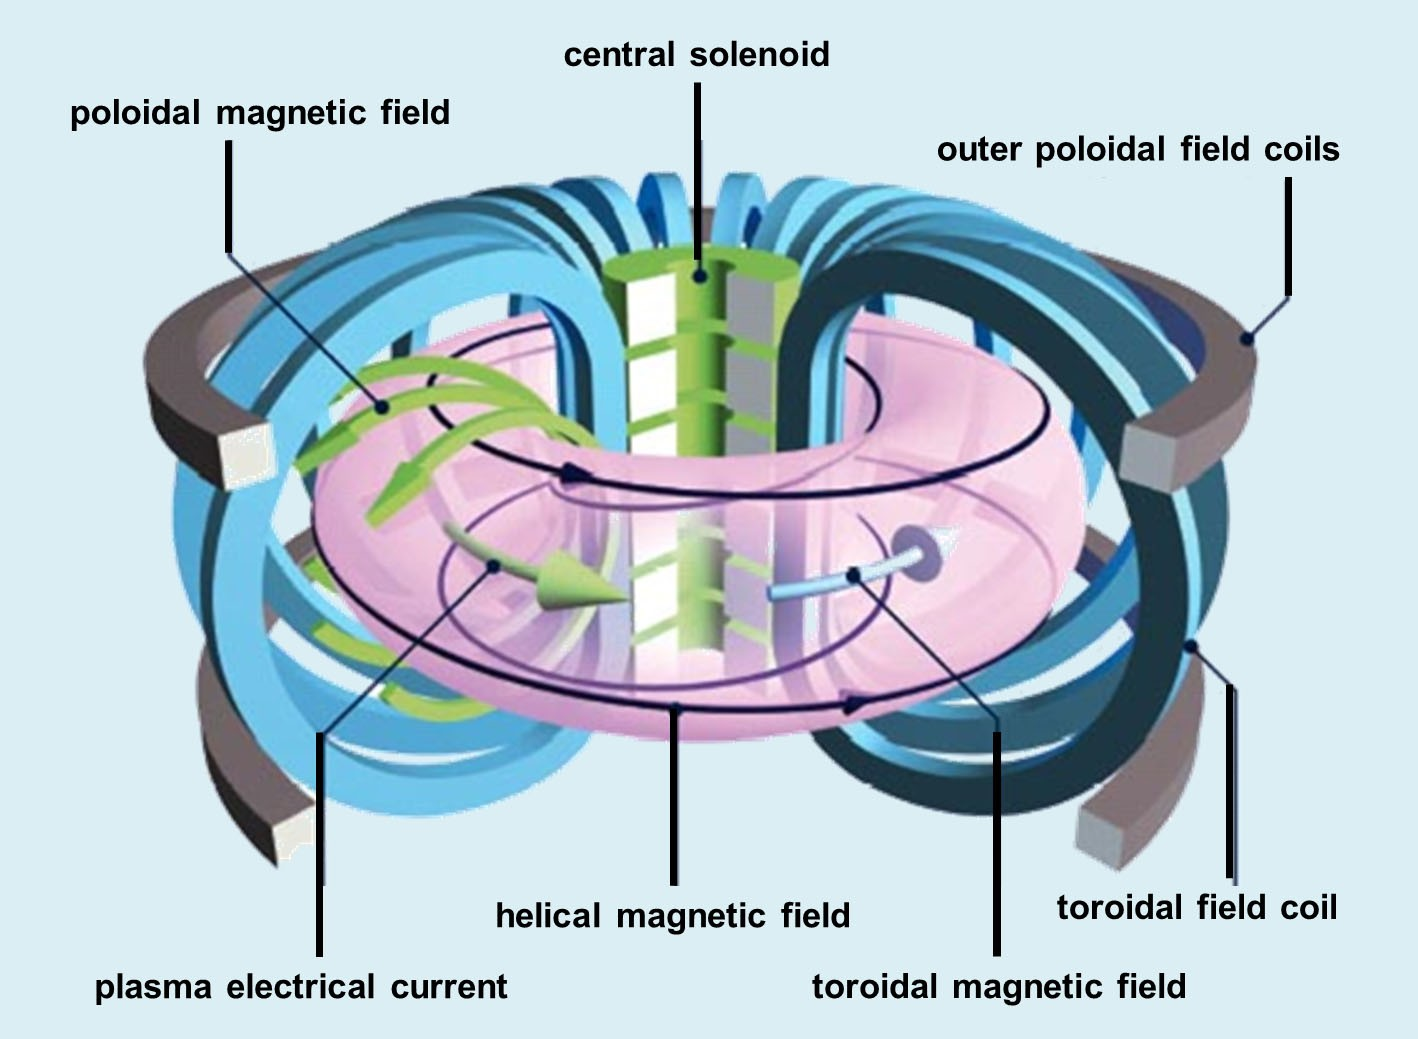
\includegraphics[scale=0.071]{./src/tokamak}
		\caption{}
		\label{subfig:tokamak}
	\end{subfigure}
	\begin{subfigure}{0.3\linewidth}
                \centering
                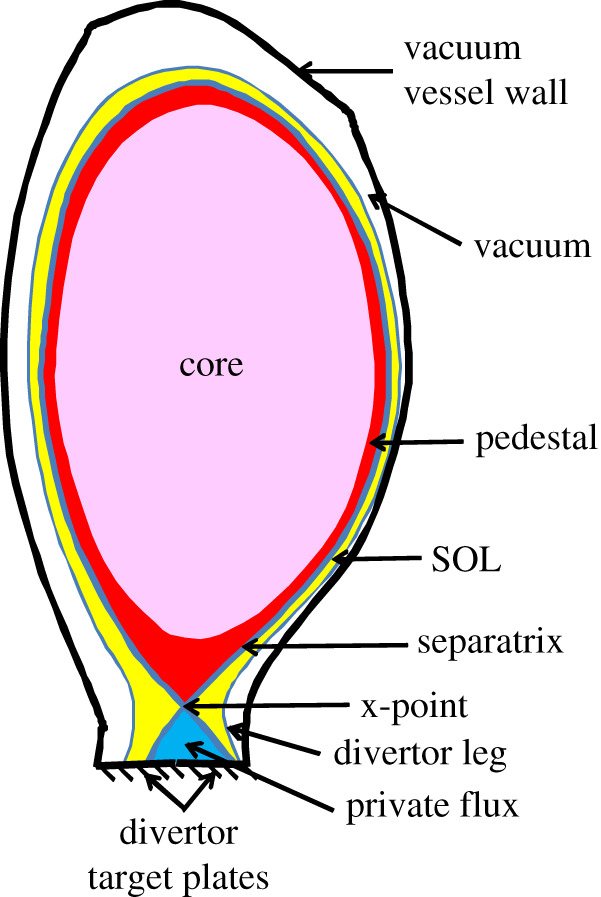
\includegraphics[scale=0.4]{./src/rsta20170435f06}
                \caption{}
                \label{subfig:cross_section}
        \end{subfigure}
	\begin{subfigure}{0.33\linewidth}
                \centering
                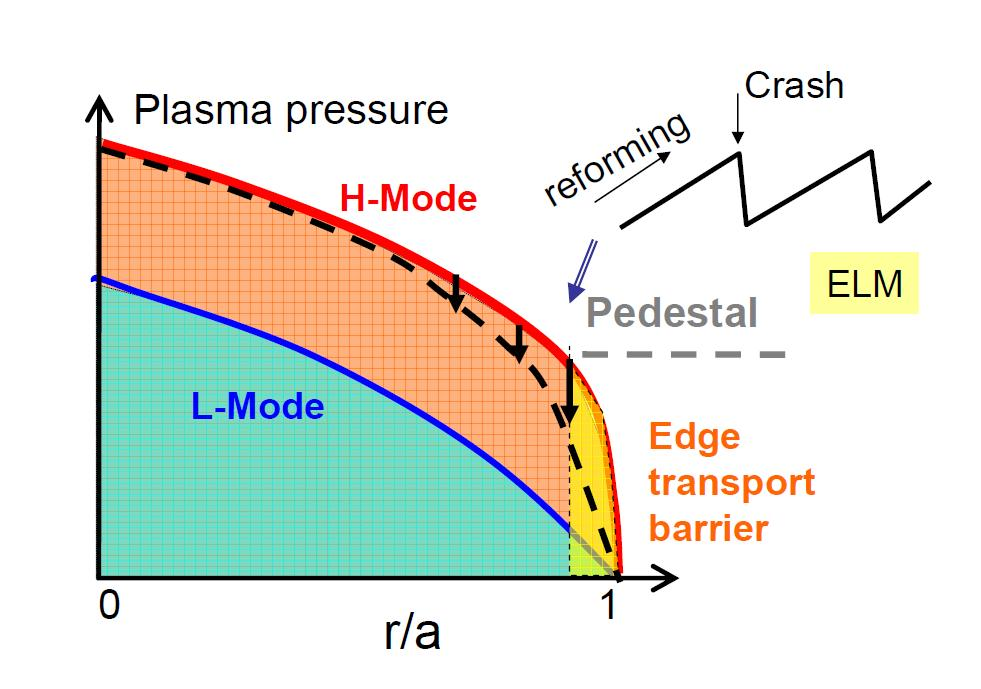
\includegraphics[scale=0.15]{./src/ELM}
                \caption{}
                \label{subfig:ELM}
        \end{subfigure}
	\caption{}
	\label{fig:tokamak_outline}
\end{figure}
\end{comment}

\subsection{JET Pedestal Database}
\begin{figure}
	\centering
	\begin{subfigure}{0.495\linewidth}
		\centering
		\includegraphics[scale=0.4]{example-image-a}
	\end{subfigure}
	\begin{subfigure}{0.495\linewidth}
		\centering
		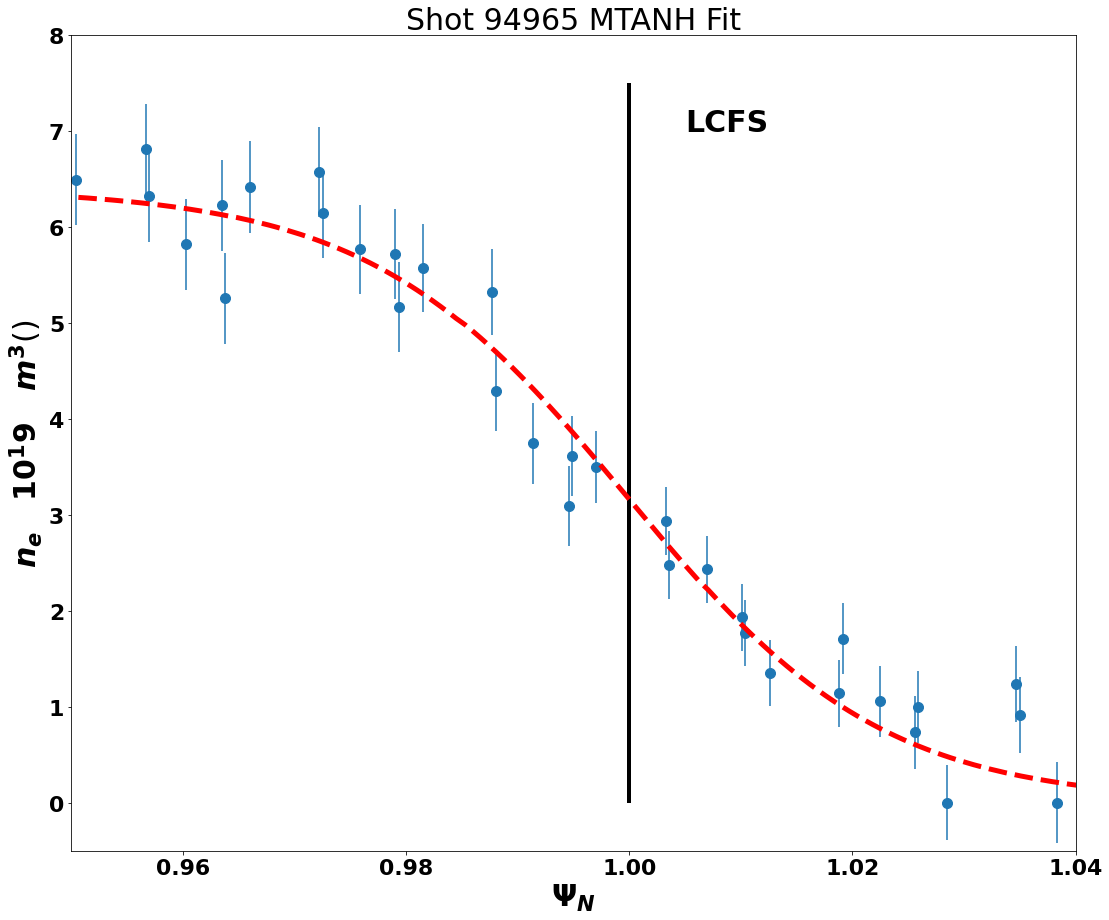
\includegraphics[scale=0.2]{./src/MTANH_fit}
	\end{subfigure}\hfill
	\caption{ \textbf{Left:} A shaping figure showing r,a, triangularity. Resembles a bow \textbf{Right:} HRTS measurement profiles (blue) radially shifted to have $T_e \approx 100$ eV at the seperatrix (LCFS). The profiles are fitted in real space using the mtanh equation \ref{eq:mtanh} then mapped to the normalized poloidal flux coordinate $\Phi_N$ (red).}
	\label{fig:pedestal_db_figs}
\end{figure}

The JET pedestal database is the most comprehensive of all pedestal databases today, containing over 3000 entries [\textcolor{blue}{Frassinetti 2021}].
Each entry corresponds to time averaged measurements of various plasma parameters over the course of 70-95\% of an ELM cycle [\textcolor{green}{cross check}].
The measurements are done using high resolution thomson scattering (HRTS)[\textcolor{blue}{Frassinetti}], and are then fitted using the mtanh function (eq \ref{eq:mtanh}). This process is visualized in Figure \ref{fig:pedestal_db_figs}. 
Since the measurements are taken near the end of the ELM cycle, the pedestal parameters should be saturated near their maximum, right before the ELM.
\begin{equation} \label{eq:mtanh}
mtanh(r) = \frac{h_1 - h_0}{2} \left( \frac{(1 + sx) e^x - e^{-x}}{e^x + e^{-x}} + 1\right) + h_0 , x=\frac{p-r}{w/2}
\end{equation}

The key engineering quantities in the database and their units are listed below, where a dimensionless unit is written as [-]. The domain of each parameter is listed in Table \ref{tab:main_domain}. 

\begin{wraptable}{r}{0.4\textwidth}
\vspace{-10pt}
\centering
\caption{Main engineering parameter domains of the filtered dataset.}
\label{tab:main_domain}
\begin{tabular}{| c | c | }
	\hline
	Eng. Param & Domain \\
	\hline
	$I_P$ [MA] & $[0.81, 4.48]$ \\
	$B_T$ [MW] & $[0.97, 3.68]$ \\
	$a$ [m] & $[0.83, 0.97]$ \\
	$\delta$ [-] & $[0.16, 0.48]$ \\
	$M_{eff}$ [-] & $[1.0, 2.18]$ \\
	$P_{NBI}$ [MW] & $[10^{-3}, 32.34]$ \\
	$P_{ICRH}$ [MW] & $[0, 7.96]$ \\
	$P_{TOT}$ [MW] & $[3.4, 38.22]$ \\
	$V_P$ [m$^3$] &  $[58.3, 82.19]$ \\
	$q_{95}$ [-] & $[2.42, 6.04]$ \\
	$\Gamma$ [$10^{22}$ e/s] & $[0, 15.5]$ \\
	$H$ [-] & $[0, 0.18]$ \\
	$\Gamma_{SD}$ [$10^6$nbar] & $[0,1000]$ \\
	\hline
\end{tabular}
\vspace{-8pt}
\end{wraptable}
\begin{itemize}
	\item $I_P$ [MA], plasma current, current driven through the plasma that generates the poloidal magnetic field
	\item $B_T$ [T], toroidal magnetic field 
	\item $R$ [m], major radius of the plasma
	\item $a$ [m], minor radius of plasma
	\item $\delta$ [-], triangularity, normalized horizontal displacement of the top/bottom of the plasma from the main axis
	\item $V_P$ [m$^3$], the plasma volume
	\item $H$, isotope ratio of fuel
	\item $q_{95}$ [-], safety factor at the flux surface edge, where safety factor is the 'windiness' of the magnetic fields in a reactor, i.e., the  number of toroidal circles the helical field line completes within one poloidal revolution, trouble arises well before $q_{95}$ reaches 1, so devices typically operate within a range of $q_{95} \in [3, 4]$ in order to maintain stable plasmas.
	\item $P_{NBI}$ [MW], neutral beam injection heating power
	\item $P_{ICRH}$ [MW], ion cyclotron radio frequency heating 
	\item $P_{TOT}$ [MW], total power ($P_{TOT} = P_{NBI}+ P_{ICRH} + P_{OHM} - P_{SH}$, where $P_{OHM}$ is the ohmic heating due to the plasma current, and $P_{SH}$ is the power lost due to the shine through of NBI heating)
	\item $\Gamma$ [ $10^{22}$ electrons per second], gas fuelling rate of the main determined fueld for the shot, this changes depending on what type of fueling is used 
	\item $DC$, the divertor configuration, can take on values of C/C, V/H, V/C, V/V, C/V, C/H, (see \textcolor{blue}{frasineeti} for more information)
	\item $TW$, the type of wall, as JET was upgraded in the mid 2010s, and moved from having a Carbon wall to an 'ITER like wall' (ILW) [SOURCE]
	\item $\Gamma_{SD}$ [$10^6$ nbar], the subdivertor pressure [SOURCE]
\end{itemize}

For the main engineering parameters, the uncertainties are calculated by taking the standard deviation of the values over the time period in which the measurements were taken. 

The global parameters stored in the database are listed below: 
\begin{itemize}
	\item $\beta_\theta^{ped}$ [-], $\beta$ is the ratio of plasma pressure $p$ to the pressure exerted by the magnetic field $B$, $\beta = p / B^2 / 2\mu_0$, thus $\beta_\theta^{ped}$ is the pressure due to the poloidal magnetic field $B_\theta$ and plasma pressure at the pedestal $p_e^{ped}$
	\item $\beta_N$, normalized $\beta$ for comparison between reactors, as $\beta$ has an inherent limit based on MHD stability, and is a function of the plasma current, minor radius and magnetic field such that $\beta_N = \beta / I / aB$, is commonly known as the Troyon factor
	\item $Z_{eff}$, the effective charge state of the plasma
\end{itemize}

The global parameters are certainly interesting, but within the context of this thesis are not considered to be viable inputs to a predictor, as they rely on information that is unavailable as a control knob on a reactor.
A truly predictive model cannot take plasma parameters as inputs. Today, EPED takes $\beta$, $n_e^{core}$ and $Z_{eff}$ as inputs assuming the feedback can be used to choose the density and $\beta$.
Models like EPED rely on the principle that reactor operators would 'know' these density and beta points are within reachable operational space, and that furthermore they know the recipe to get there.
A model of interest would be that which uses the main engineering parameters to calculate profile parameters like height, width, or position for the pedestal quantities temperature, density, or pressure.
The pedestal profile parameters stored in the database are determined using the mtanh fit (equation \ref{eq:mtanh}), and the uncertainties are the fit uncertainties from the use of the mtanh function [\textcolor{blue}{SOURCE}].
The fit uncertainties are expected to be significantly smaller than the natural scatter of the data due to the fluctuation of the plasma.

Additionally, there exist so called FLAGS, which correspond to the specific setup of an experiment.
For example, what element the fuel is, if resonant magnetic pulses (RMPs) [\textcolor{blue}{source}], pellets [\textcolor{blue}{source}] or impurity seeding [\textcolor{blue}{source}] were used are all FLAGS contained in the database.
Additionally, there is a flag corresponding to the quality of the HRTS measurement, as each entry is validated either by hand or computationally.
Only entries that have been validated are used in this thesis.
Shots with impurity seeding are used, as they make up about 600 entries.
RMPs, pellets, and kicks are used to manipulate the pedestal for ELM control, mitigation, or suppression [\textcolor{blue}{Viezzer NF 2018}].
To keep the dataset simple in this thesis, these entries are excluded.
After filtering out the RMPs, Kicks, Pellets, non-validated HRTS, and shots that do not use deuterium, the dataset is reduced to 1888 entries. The final pedestal parameter domains are given in the table below.
\begin{center}
\begin{tabular}{ | c | c | c | c | c | }
	\hline 
	& Height & Width ($\Psi_N$) & Position ($\Psi_N$) & Slope (-) \\ 
	\hline
	$n_e^{ped}$ &[1.849, 11.737] ($10^{19}$ m$^3$) & [0.015, 0.173]& [0.953, 1.029] & [$10^{-6}$, 0.188] \\
	$T_e^{ped}$ & [0.149, 1.894] (keV)& [0.013, 0.105] & [0.926, 1.002] & [0.026, 0.502] \\
	$p_e^{ped}$ & [0.808, 17.804] (kPa)& [0.014, 0.099] & [0.931, 1.002]& [0.041, 0.789] \\
	\hline
\end{tabular}
\end{center}


\subsubsection{Empirical Analysis}
\begin{figure}
        \centering
        \begin{subfigure}{0.5\linewidth}
                \centering
                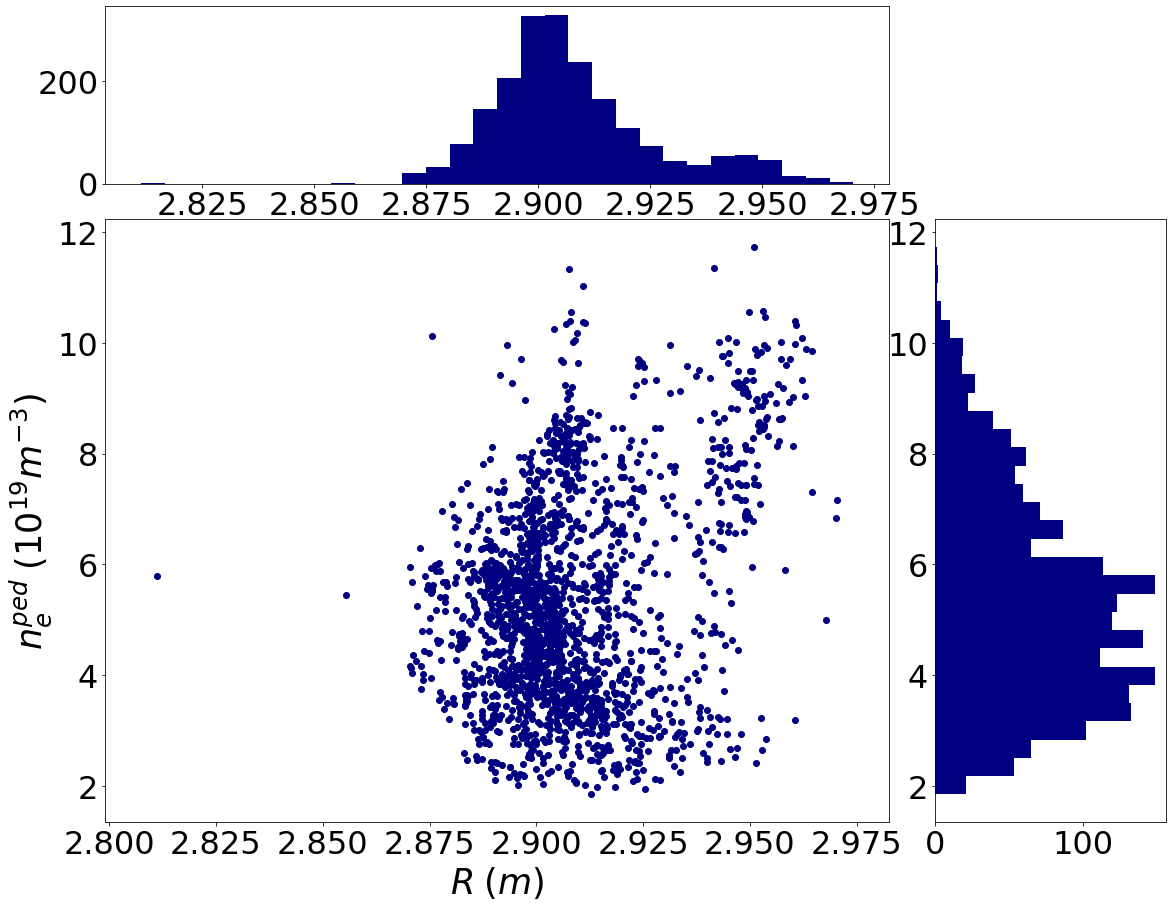
\includegraphics[scale=0.2]{./src/R_vs_NEPED_matplotlib}
                \caption{}
                \label{subfig:rvsneped}
        \end{subfigure} \hfill
        \begin{subfigure}{0.45\linewidth}
                \centering
                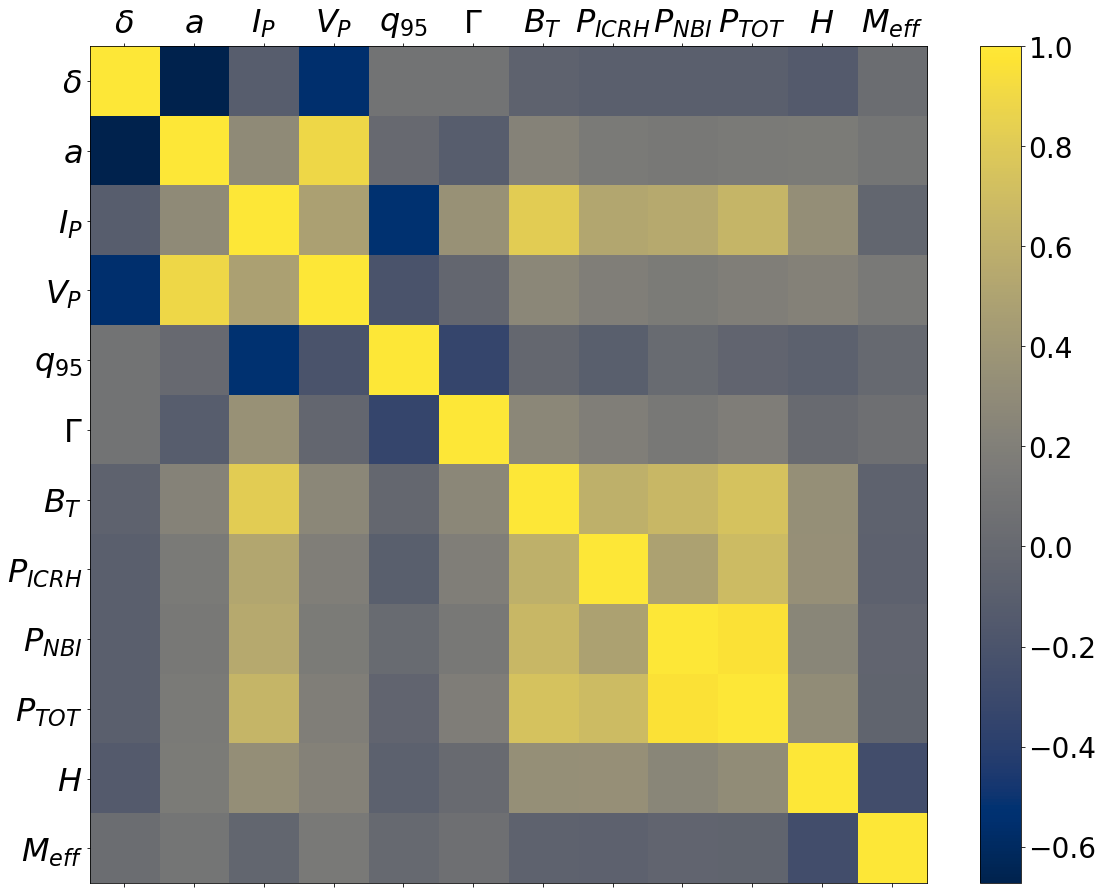
\includegraphics[scale=0.2]{./src/input_correlations}
                \caption{}
                \label{subfig:corr_shit}
        \end{subfigure}
	\caption{Emperical data plots of the JET pedestal database. \textbf{Left:} the 'ice cream corerlation' between the major radius $R$, divertor configuration, and $n_e^{ped}$,  \textbf{Right:}  correlation matrix of the main engineering parameters. A grey coloring represents no correlation, whereas blue and yellow are negative and positive correlation respectively.}
	\label{fig:emperical}
\end{figure}
Empirical analysis of the JET pedestal database has been done [\textcolor{blue}{SOURCE LORENZO DB SHIT}], and has yielded the following log-linear scaling law for the pedestal density height $n_e^{ped}$.
\begin{equation} \label{eq:scaling}
	n_e^{ped} = (9.9 \pm 0.3) I_p^{1.24 \pm 0.19} P_{TOT}^{-0.34 \pm 0.11} \delta^{0.62 \pm 0.14} \Gamma^{ 0.08 \pm 0.04} M_{eff}^{0.2 \pm 0.2}
\end{equation}
In this thesis, we will take the pedestal prediction with ML approaches relative to the performance of the empirical scaling law as the well defined focus for the project.
The choice of parameters from the log-linear regression by Lorenzo et. al., was backed by physical intuition about what drives the pedestal density height. Since log-linear regression was used, it is also assumed that the scaling law above avoided using cross-correlated variables, which can verified in Figure \ref{subfig:corr_shit}. 

In order to improve prediction quality, it may prove useful to include additional inputs from the list of main engineering quantities that were not used in the log-linear scaling.
However, by plotting joint histograms between the control parameters and $n_e^{ped}$, some serious questions can be raised regarding which parameters can and should be given to a machine learning model.
For example, looking at the dependence of the major radius $R$ in Figure  \ref{subfig:rvsneped}, one could jump to early conclusions and say that with higher values of $R$, a higher pedestal height is achieved!
However, this is a case of ice-cream correlation\footnote{ice cream correlation refers to the correlation of increasing ice cream sales and increasing number of drownings in Finland during the summer. Although the variables are indeed correlated, higher ice cream sales are not in fact the causation of higher drowning rates, nor vice-versa.}, and the real culprit of the causation is the Shafranov shift; the outward radial displacement of the magnetic axis from the geometric axis that is prominently found in MCF devices\textcolor{blue}{[Shafranov SOURCE]}. The shift is understood to be induced by plasma pressure, and thus is normally linear in $\beta$. Since $\beta$ and pressure are heavily dependent on the aspects of the machine, the Shafranov shift is also machine dependent. 
For this reason, $R$ is excluded from the list of inputs to the ML models in this thesis, and only when multi-machine databases are available should it be included.
The divertor configuration on the other hand, does have a real correlation, and can have a large impact on the pedestal. However, the analysis in this thesis makes use of the numerical parameters available only, and thus DC will not be used as an input parameter, as it is categorical.  

Another engineering parameter that is ignored in the analysis is the sub-divertor pressure $\Gamma_{SD}$.
From the filtered dataset, the values of the sub-divertor vary widly, with 130 entries having an error and value of 1000 [$10^6$ nbar], while having close to 500 entries that vary between [0, 0.5].
Because of this volatility, $\Gamma_{SD}$ is ignored, however future research may choose to filter the dataset such that inclusion of $\Gamma_{SD}$ is possible.



\section{General Machine Learning Analysis}\label{sec:principle-machine-learning-analysis}
Within the context of this thesis, a model refers to a prediction function $f$ that takes any combination of the main engineering parameters as inputs, $\vec{x} = (x_1, x_2, \cdots, x_p)$,  and provides an estimate of the pedestal density height, $\hat{y}$, as well as the uncertainty of the estimate (when applicable).
The prediction quality is quantified through both RMSe and MAE, since a robust model minimizes both of these.
The RMSE penalizes predictions that are far away from the ground truth, whereas the MAE calculates a uniform distance between the prediction and the ground truth.
\[RMSE = \sqrt{\frac{\sum_i^N \left( y_i - \hat{y}_i \right)^2}{N}} \quad\quad MAE = \frac{\sum_i^N |y_i -  \hat{y}_i |}{N}  \] 
where $N$ is the number of points predicted upon, and $y_i$ is the ground truth value of $n_e^{ped}$ for the $i$'th entry in the dataset. 
\subsection{Model Fitting and Validation}
To make a prediction, the model must first be \textit{fitted}, which means to learn the parameters $\vec{\theta}$ of the prediction function using a model specific learning algorithm such that $f = f(\vec{x}: \vec{\theta})$.
In the case of linear regression, the learning algorithm is the ordinary least squares method (OLS) [SOURCE] which minimizes the mean squared error in order to find the optimal linear coefficients $\theta(w_i)$.
Not all supervised learning regression algorithms minimize the RMSE or MAE to fit model parameters.
The RMSE and MAE as stated above are merely a quantization of the performance of a particular model.

The scoring of the performance of a fitted model shall be made using data that the model had previously not seen.
If this were not the case, the model would simply repeat what it had been fitted with, and would fail to predict useful information on yet unseen data.
This is called \textit{overfitting}; to avoid overfitting a common practice in supervised machine learning is to hold out part of the available data as a test set.
This can be done by randomly splitting the available data into training and test subsets, and to evaluate the model on the test set.
Then, depending on the performance, adjust the \textit{hyperparameters} of the model (an example of a hyperparameter is the number of trees in a random forest, or learning rate for ANN's) in order to optimize the performance on the test set.
However, this runs into the problem of overfitting on the test set, since the hyperparameters can be adjusted until the model preforms best on the test set.
In this sense, knowledge about the test set leaks into the model, and evaluation metrics no longer report on general performance.
Additionally, in randomly splitting the data into two groups, there is a new problem of \textit{selection bias}[SOURCE], in which the model's results are dependent on the random choice of training/test sets.
To overcome these problems, \textit{cross-validation} or CV is implemented throughout the analyses in this thesis to validate the parameters and generalization capabilities of a model.
The general approach for \textit{k-fold} CV is to split the dataset into $k$ subsets, and apply the following procedure to each of the k folds:
\begin{itemize}
	\item Use $k-1$ of the folds to fit a model 
	\item Hold out the remaining fold to validate the fitted model
\end{itemize}

Furthermore, \textit{repeated k-fold} CV is employed, in which the above process is repeated $p$ times.
The final performance measure is then the average of the scores on the test sets left out.
This method is very computationally expensive since $k*p$ models are being fit, but it is extremely efficient with the data, while additionally removing selection biases with sufficient folds and repeats.

\subsection{Linear Regression}
Up to now, the plasma physics community has used log-linear regression to create scaling laws like that from Lorenzo et. al.
A general overview of Linear Regression can be found [SOURCE]. 
Additional details that are used in this thesis are as follows: 
\begin{itemize}
	\item By minimizing the MSE through OLS, the scalar linear coefficients $w_i$ corresponding to the control parameter $x_i$ can be determined, and from these coefficients we learn the linear correlation of an engineering parameter and $n_e^{ped}$, i.e., if the coefficient in front of the plasma current, $w_{I_P}$, is positive, then as $I_P$ increases, so will the prediction of $n_e^{ped}$.
	\item By adding a regularization term ($L^1$ norm of the weights) to the MSE cost function, the coefficients will be minimized as well, resulting in some coefficients becoming 0. From this it can be determined if a engineering parameter is 'useful' in the context of predicting point estimates of $n_e^{ped}$ using linear regressors, and can reduce dimensionality when possible. This is known as LASSO [SOURCE].
	\item The uncertainty in the prediction can be determined by transforming the weights from scalars into normal distributions with mean $\mu$ centered around the scalar coefficient, and spread $\sigma^2$ representing the uncertainty in the coefficient, thus transforming the point estimate into a distributional estimate. This is otherwise known as Bayesian Regression [SOURCE]. \textcolor{green}{clearer explanation}.
\end{itemize}

By using more input parameters than that which is used in the scaling law \ref{eq:scaling}, the hope is to achieve a better RMSE while additionally maintaining interpretability, i.e., attach physical intuition behind why the determined coefficients are the way that they are.
We do not expect any new revelations from the coefficients determined by a linear regressor using more engineering parameters than that listed in \ref{eq:scaling}, i.e., the pedestal density will still increase as the plasma current increases. The linear models analysed come from the sklearn library. 

\subsection{Gaussian Processes}
In contrast to linear models, Gaussian Processes (GPs) are non-parametric, in that there is no function to be minimized, but rather an optimal set of functions is to be found that best characterize predicting $n_e^{ped}$ given the engineering parameters as inputs.
Much more can be read about GPs in the following sources [SOURCES].
The details pertinent to the analysis in this thesis are as follows:
\begin{itemize}
	\item Choice of kernel (covariance function) is normally based on the 'wigglieness' of the functions one is trying to parameterize[SOURCE], but with higher dimensional space, this means nothing. Therefore the kernels sought after are those that when optimized give best predictions of the pedestal density.
	\item Prediction uncertainty is built into GPs as the joint-gaussian group of functions determined through optimization of the kernel will give predictions of the pedestal density that are averaged for the point prediction, and the standard deviation is the uncertainty. 
	\item Sensitivity analysis is used to determine the relevant engineering parameters for GPs, from which the dimensionality of the input space can be reduced if parameters are deemed irrelevant. Three different forms of sensitivity analysis used: KLD, ARD, VAR[SOURCE], which all make use of thte length-scale parameters of the kernel in a GP model. The KLD, ARD, and VAR are outlined below. 
	\item To utilize the measurement uncertainties given in the database, there are two approaches: (a) a fixed noise kernel is added on to the base kernel[SOURCE] such that the measurement uncertainties are additive to the input space. (b) Transforming the GP model from homoscedastic to heteroscedastic, where the homoscedastic model assumes constant guassian noise and the heteroscedastic takes noise values that vary for each input entry. Furthermore, the heteroscedastic model attepmts to learn the uncertainty space given the uncertainty inputs, i.e., not only is the laten space of $n_e^{ped}$ mapped, but also the uncertainty latent space of $n_e^{ped}$.   
\end{itemize}

GPs scale horribly with increasing input space size, therefore the hope of using sensitivity analysis is to remove any engineering inputs if they do not improve the prediction capability of them GP model.

Additionally, since the each variable used in the fitting procedure is numerical, there exists no urgent need to try out different combinations of kernels, i.e., multiplying or adding kernels together is not analysed in this work, but something to try in the future. 

The three types of sensitivity analysis used:
\begin{itemize}
	\item Automatic Relevance Determination (ARD): The predictive relevance of each input variable is infered from the inverse of the length-scale parameter associated with that variable within the kernel. A large length scale (infinite for example) means that no correlation between the latent space and the variable in question, and thus the relevance would be zero \textcolor{blue}{SOURCE paananen}. 
	\item Kullback-Leibler Divergence (KLD): The KLD is a well known measure of dissimilarity between two probability distributions, and is a function of both the latent mean and uncertainty of each distribution \textcolor{blue}{SOURCE Kullback Leibler 1951}. In this case, the input space is 'shifted' via the pertubation of a single variable's values, and the KLD of the resulting new latent space is measured against the unperterbed case. A large change in the KLD indicates that the single variable that was perturbed has high prediction relevance.  [\textcolor{blue}{SOURCE paananen}]
	\item Variance of the Posterior (VAR): The same method of perturbation applies, but instead of calculating the KLD, variability in  only the latent mean of the fitted GP is calculated. [\textcolor{blue}{SOURCE paananen}]
\end{itemize}

The gaussian process models used in analysis are adapted from the GPy libarary. 

\subsection{Random Forests}
Another popular non-linear model is the ensemble of decision trees [SOURCE] that is the Random Forest(RF). More can be read about here [SOURCE], but the details pertinent to the thesis are stated below.
\begin{itemize}
	\item RFs are fitted using boostrap aggregation (bagging). Each decision tree within the forest is fit from a 'bag' of random samples drawn from available training entries, meaning not every tree will see every available training sample, allowing for the calculation of the average error for each sample using the predictions of trees that do not contain the sample in their bag. This allows us to approximate how many decision trees to use in the forest, as the OOB error will eventually stabalize. The bag consists of a pre-determined number of features which are also randomly sampled, which allows for the determination of the optimal number of inputs to sample, as well as which inputs are optimal.  [\textcolor{blue}{Elements of Statistical Learning p592}]
	\item UQ in prediction can be determined by taking the standard deviation of predictions from all of the decision trees that make up the forest. 
	\item A variant of RFs called Extremly Randomized Trees (ERTs) will also be compared. The two main differences between RFs and ERTs are (a) decision trees in ERTs sample entries for their bags without replacing such that no decision tree contains any the same entries and (b) nodes in decision trees are split based on different critera; RFs convert parent nodes into two homogeneuos nodes by choosing the split that minimizes the MSE, whereas ERTs convert the parent node into two child nodes via a random split. [\textcolor{blue}{ERTs Pierre Geurts 2006}]
\end{itemize}

Random Forests and Extremely Randomized Trees offer little interprability in comparison to parametric models, but by quantifying how much the impurity of a node decreases (a pure node has no child nodes) with the probability of reaching that node, the relative importance of the feature housed in the node is determined. Using this, we can get insight into which features are driving the predictions of $n_e^{ped}$ for RFs and ERTs. The RFs and ERTs used in this analysis are adapted from the sklearn library. 

\subsection{Artificial Neural Networks}

Numerous previous studies have investigated the reasons to which why artificial neural networks (ANNs) work [\textcolor{blue}{SOURCE}].
Since ANNs are very delicate, the primary goal in this thesis is to probe the hypereparameter and architecture spaces for future research to build on top of.
The ANNs used in this thesis are all fully-connected feed-forward networks[SOURCE].
Work has already started on using ANNs in predicting pedestal quantities, \textcolor{red}{METNION ANDREAS SOMEHOW}.
\begin{itemize}
	\item Hyperparameter \& Architecture search: mini-batch size, learning rate,  number and size of hidden layers, activation functions, layer types (dense, cross), length of training, regularization (batch normalization, weight decay), early stopping. The optimal hyperparameters and architectures determined are those that achieve the lowest RMSE through the cross-validation process.
	\item Prediction uncertainty is obtained through ensembling many ANNs of similar architectures such that the standard deviation of all the predictions in the ensemble is the uncertainty in the ensemble prediction.
\end{itemize}

The ANNs used in this analysis are built using pytorch. 

\subsection{Meta-Modeling}
Another use of the uncertainties stored within the database is for a given entry to generate normal distributions with mean of a parameter value and spread of the uncertainty, and by sampling from the generated distribution, it is possible to create new 'synthesized' entries.
As seen in the next section, many models can predict well for $n_e^{ped} \leq 10$, but struggle for densities higher than that.
By including synthesized values in the fitting procedure the hope is that models would be able to predict better for the higher $n_e^{ped}$ values.

\section{Results}{\label{sec:results_1}
Each model analysed is fit using the following list of main engineering parameters as inputs:
\begin{itemize}
        \item $I_p, B_T, a, \delta, M_{eff}, P_{NBI}, P_{ICHR}, P_{TOT}, q_{95}, \Gamma, H, V_P$.
\end{itemize}
Through the use of cross-validation, the hyperparameters of each model are tuned such that optimal performance is achieved on the average performance on each fold subset.
The relevant hyperparameters, and how they were determined is discussed in each indivdual model subsection, as well as the effect of meta-modeling when applicable.
Table with performance metrics for optimal hyperparameters for each model can be found in Table \ref{tab:performance_models}.

\subsection{Linear Regression}
A linear regression model without an intercept was fit using the 'as is' control parameters as inputs, and we can see in Figure \ref{fig:lin_reg} that by including more parameters than the original 5 used in the scaling law that the RMSE and MAE improve. 

\begin{wraptable}{r}{0.36\linewidth}
\centering
\vspace{-15pt}
\caption{Coefficients determined by Bayesian Linear Regression. Each coefficent is a normal distribution with mean $\mu$ and spread $\sigma^2$}\label{tab:new_coef}
\begin{tabular}{ | c | c | c |}
			\hline
			Feature & $\mu$ & $\sigma^2$ \\
			\hline
			$I_p$ & 0.15 & 0.06 \\
			$B_T$ & 0.956 & 0.072 \\
			$a$ & 2.966 & 0.479 \\
			$\delta$ & 12.95 & 0.154 \\
			$V_P$ & -0.05 & 0.007 \\
			$q_{95}$ & -1.064 & 0.0542 \\
			$P_{NBI}$ & $-1.911$ & 0.0546 \\
			$P_{ICRH}$ & -1.976 & 0.0561 \\
			$P_{TOT}$ & 1.926 & 0.0557 \\
			$\Gamma$ & 0.125 & 0.007 \\
			$H$ & -4.016 & 0.374  \\
			$M_{eff}$ & 1.369 & 0.053 \\
			\hline
\end{tabular}
\end{wraptable}

Through the use of regularization via the LASSO method, the following features were deemed 'unimportant' (their coefficients dropped to 0 or near 0): $H, M_{eff}, B_T, V_P$.
A new model with reduced dimensionality was fit by removing the unimportant features from the input space and it was seen that the prediction quality decreased dramatically with any reduction of dimensionality; in removing H or $M_{eff}$ from the input space, the RMSE and MAE increased to much above that of the scaling law, while when removing $V_P$ or $B_T$, there was an increase of 1.5 in the RMSE and MAE. 
The results of LASSO can be slightly misleading, as linear regressors and their regularized extensions are prone to problems when working with many correlated variables. and many of the variables in the input space are correlated (e.g., $P_{TOT}, P_{NBI}, P_{ICRH}$), which may be why the best RMSE and MAE are achieved when all variables are included.

Fitting a Bayesian Ridge regressor using all of the available engineering parameters yielded new coefficients (as well as the uncertainties therewith), which can be seen in Table \ref{tab:new_coef}. 
From the coefficients and their uncertainties, the general uncertainty in the point prediction of $n_e^{ped}$ can be ascertained. The uncertainties were normally distributed and range from 1.64 to 1.8 ($10^{19}\text{m}^{-3}$). Having high uncertaity is good when the prediction is far from the ground truth (high residual), but for predictions on $n_e^{ped} \geq 8.5$ the uncertainty no longer covers the residual. 
Just like the scaling law, the predictions from the Bayesian linear model taper off at around $n_e^{ped} \geq 8.5$, which suggests that parametric models like linear regressors are generally unable to capture the hidden secrets of higher pedestal density heights from the given set of input parameters.
\begin{figure}
	\centering
	\begin{subfigure}{0.495\linewidth}
		\centering
		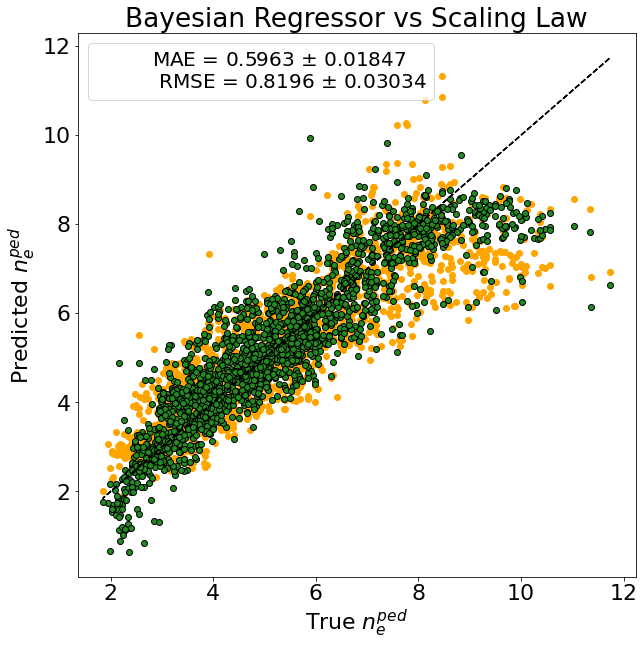
\includegraphics[scale=0.35]{./src/Baysian_regression_predictions}
	\end{subfigure}
	\begin{subfigure}{0.495\linewidth}
		\centering
		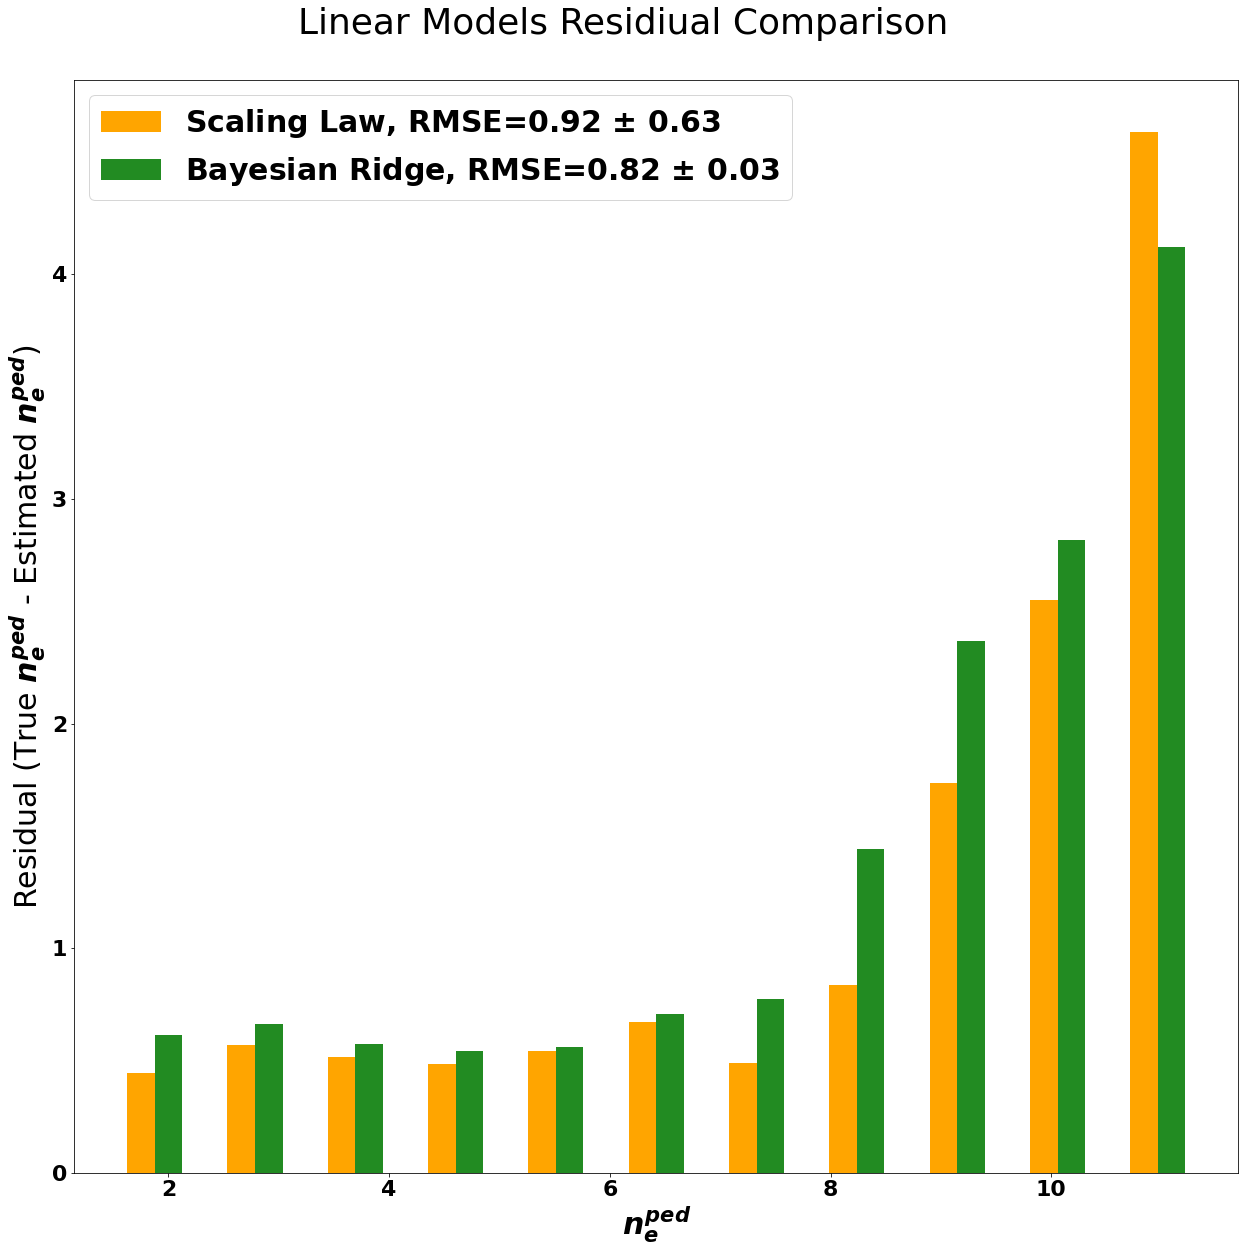
\includegraphics[scale=0.18]{./src/linear_comp}
	\end{subfigure}\hfill
	\caption{Comparison of a Bayesian Ridge Regressor fit using all available engineering parameters against the log-linear scaling law give in \ref{eq:scaling}. \textbf{Left:} The predictions of a Bayesian Regressor (green) vs the scaling law (orange) with the ground truth being the black dotted line. \textbf{Right:} The Residual comparison of the bayesian regressor (green) and the scaling law (orange) }
	\label{fig:lin_reg}
\end{figure}

\begin{comment}
\begin{figure}
	\begin{floatrow}
		\ffigbox{
		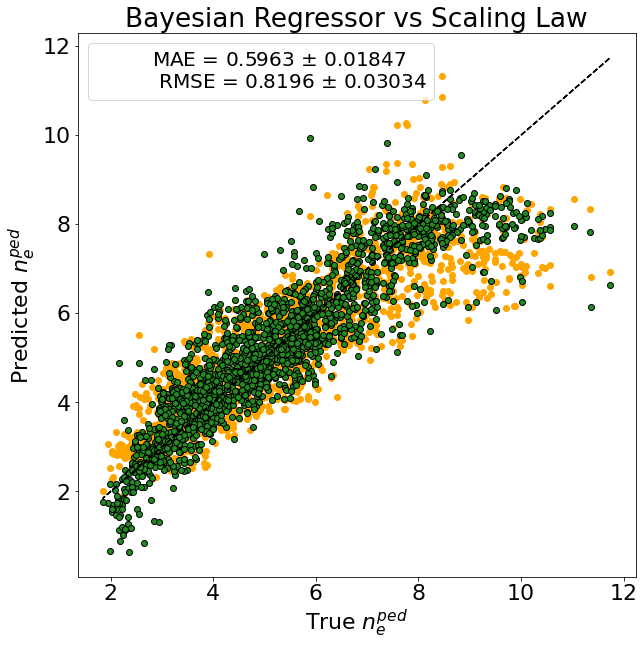
\includegraphics[scale=0.3]{./src/Baysian_regression_predictions} 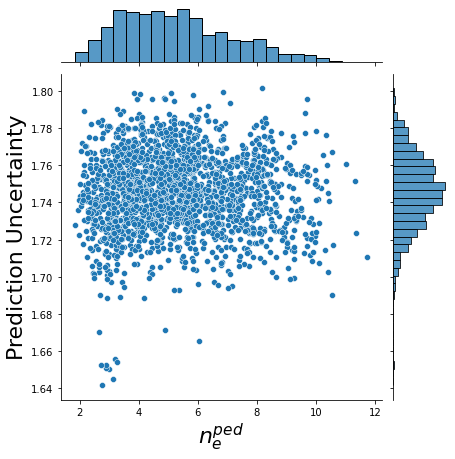
\includegraphics[scale=0.35]{./src/Baysian_regression_uncert}}{
		\caption{Predictions using the coefficients in the table on the RHS compared to the scaling law} \label{fig:linreg}}
		\capbtabbox{
				\begin{tabular}{ | c | c | c |}
			\hline
			Feature & $\mu$ & $\sigma^2$ \\
			\hline
			$I_p$ & 0.15 & 0.06 \\
			$B_T$ & 0.956 & 0.072 \\
			$a$ & 2.966 & 0.479 \\
			$\delta$ & 12.95 & 0.154 \\
			$V_P$ & -0.05 & 0.007 \\
			$q_{95}$ & -1.064 & 0.0542 \\
			$P_{NBI}$ & $-1.911$ & 0.0546 \\
			$P_{ICRH}$ & -1.976 & 0.0561 \\
			$P_{TOT}$ & 1.926 & 0.0557 \\
			$\Gamma$ & 0.125 & 0.007 \\
			$H$ & -4.016 & 0.374  \\
			$M_{eff}$ & 1.369 & 0.053 \\
			\hline
		\end{tabular}
		}{\caption{The coefficient distribution parameters determined from Bayesian Linear Regression. Each coefficent is a normal distribution with mean $\sigma$ and spread $\sigma^2$}\label{tab:new_coef}}
		\end{floatrow}
	\end{figure}
\end{comment}
\subsection{Gaussian Process}

To determine the results of sensitivity analysis, a GP model with a RBF kernel with added constant bias term is setup and fitted using all of the available parameters. The model is optimized to the maximum of the marginal likelihood, and the relevance of each variable is calculated using ARD, KLD, and VAR. This process of optimization is repeated 5 times and the results over all 5 are averaged. We can see in Figure \ref{fig:GP_dim} that each method gives relatively similar results, and the order of importance of the three methods averaged is relisted below.  
\begin{comment}
\begin{itemize}
	\item \textbf{ARD}: $\delta, a, V_P,  I_p, P_{ICRH}, \Gamma, P_{NBI},  B_T, P_{TOT}, q_{95}, H, M_{eff}$
	\item \textbf{KLD}: $\delta, a,  I_p, P_{NBI}, V_P, P_{TOT},  q_{95}, \Gamma, B_T, P_{ICRH}, H, M_{eff}$
	\item \textbf{VAR}: $\delta, a, I_p, \Gamma, V_P, P_{NBI}, q_{95}, P_{ICRH}, P_{TOT}, B_T, H, M_{eff}$
\end{itemize}
\end{comment}
\begin{itemize}
	\item  $\delta, a, I_p, V_P, P_{NBI},\Gamma, P_{TOT},  q_{95},  P_{ICRH}, B_T, H, M_{eff}$
\end{itemize}
\begin{figure}
	\begin{subfigure}{0.48\linewidth}
		\centering
		\includegraphics[scale=0.2]{ ./src/GP_sensitivity_analysis_final_v1}
	\end{subfigure}\hfill
	\begin{subfigure}{0.48\linewidth}
		\centering
		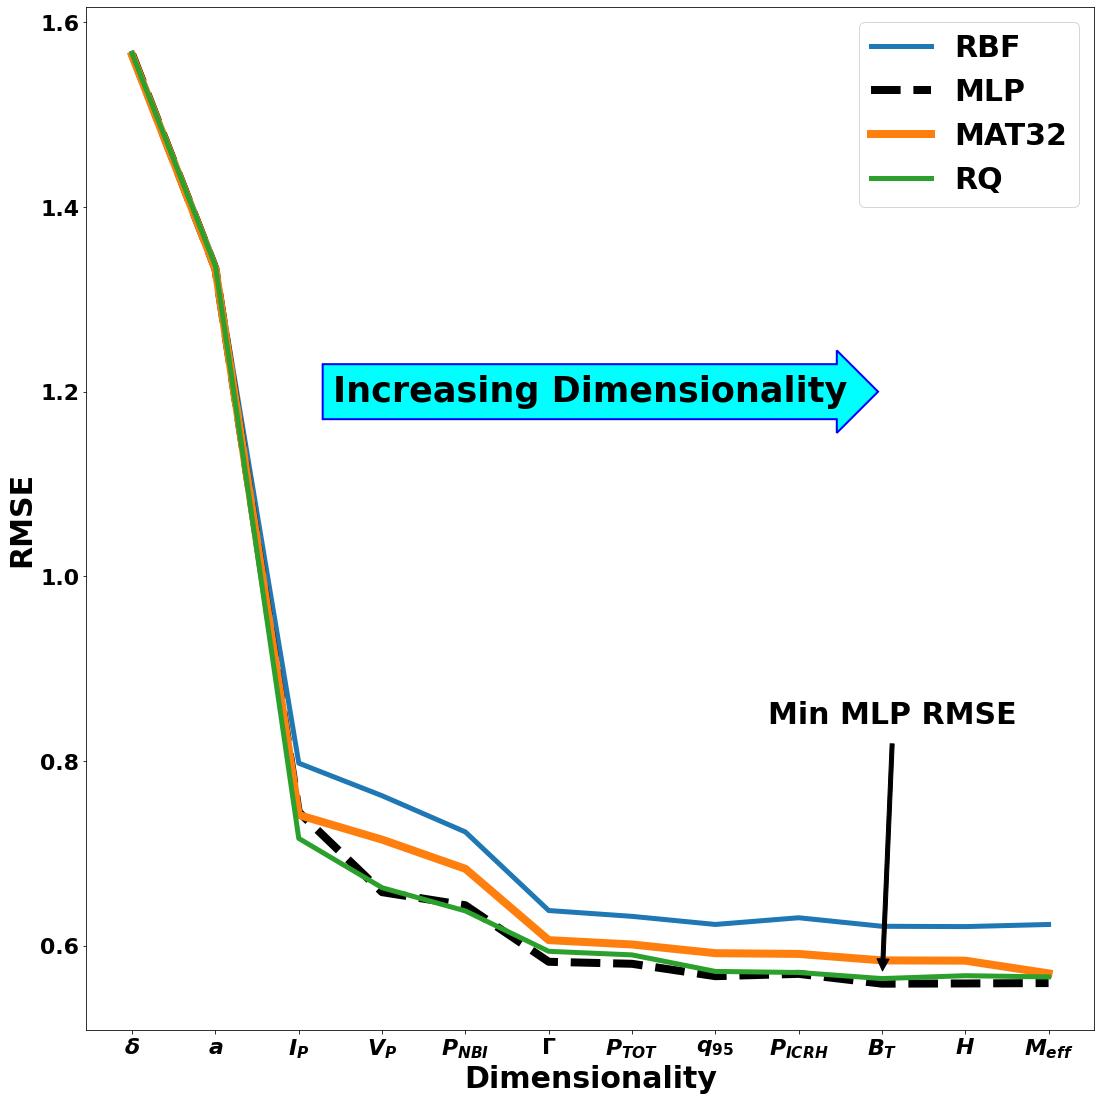
\includegraphics[scale=0.2]{ ./src/final_GP_dim_v2}
	\end{subfigure}
	\caption{Steps towards dimensionality reduction through the use of Gaussian Processes. \textbf{Left:} The result of sensitivity analysis as well as the average of the three types used plotted in the dashed black line. \textbf{Right:} The dimensionality order of input variables comes from their ranking via the average of the three sensitivity analyses (dashed black line in diagram to the left). For each kernel, a GP model is fit using cross-validation (5 folds, 5 repeats) for each additional dimension of data, starting with 1d input of $\delta$, followed by 2d input of $\delta, a$ and so on. Then the RMSE is calculated on folds left out and averaged across all folds. } \label{fig:GP_dim}
\end{figure}
The sensitivity analysis for GPs suggests that H and $M_{eff}$ do not aid in predicting the pedestal density, which may be due to the filtered dataset used for fitting being exclusive in its values for $H$ and $M_{eff}$ (only deuterium experiments were considered), 
I would expect this to change if a wider range of fuelling elements were included in the dataset, and for future work do not expect $M_{eff}$ to rank as low as it does. Each sensitivty analysis also ranks $B_T$ low, which is most likely due to the inherent correlation between $B_T, q_{95}, \text{and} I_P$, as most of the information of $B_T$ is contained within $q_{95}$. 

Using the results from the sensitivity analysis, the performance vs dimensionality was measured for four homoscedastic GPs of varying kernels and is plotted in \ref{fig:GP_dim}. It can be seen that the top performing kernels were the MLP and Rational Quadratic (RQ). We observe also that the MLP and RQ do not improve \textit{after} $B_T$ is added to the input space, i.e., confirming the results of the sensitivity analysis. This means that in regards to the current dataset, it is unnessecary to supply $H \text{ and } M_{eff}$ to a GP, which will reduce the computation time when fitting. However, this reduction can be subject to change, since, as stated before, the dataset used was exclusive in its choice of $H$ and $M_{eff}$, thus for multi machine or multi element datasets, the importance of these two variables may be more than what was found here. Nevertheless, the remainder of the GP models that are analysed in this section do not use $H$ or $M_{eff}$ during the fitting procedure. 

To determine the effect of uncertainty propagation, the two approaches described in Section 2 are applied; (a) a fixed kernel with $n_e^{ped}$ measurement uncertainties along the diagonal is added to a base kernel, (b) a heteroscedastic model is fixes the built in noise variance component of GPs to be the measurement uncertainty of $n_e^{ped}$ such to learn the latent space of the used uncertainty. This process is done for both the RQ and MLP kernel and compared to the homoscedastic models.
We see from Figure \ref{fig:MLP_UQ} that the homoscedastic slightly outpreforms the heteroscedastic model, yet their uncertainties could not be more different. As the heteroscedastic MLP model attempts to learn the uncertainty space, we can see that although the predictions for $n_e^{ped} > 10$ are furthest, its uncertainty is much lower. Since heteroscedastic GP learns the propogated uncertainties, the generated prediction functions end up being much closer to eachother, resulting in a lower variance in prediciton. This is very different from the homoscedastic and fixed models, which although perform very well, suffer from having their prediction generating functions far apart (a variance $ \geq \pm 1.2$), regardless of prediction accuracy.

\begin{figure}\centering
		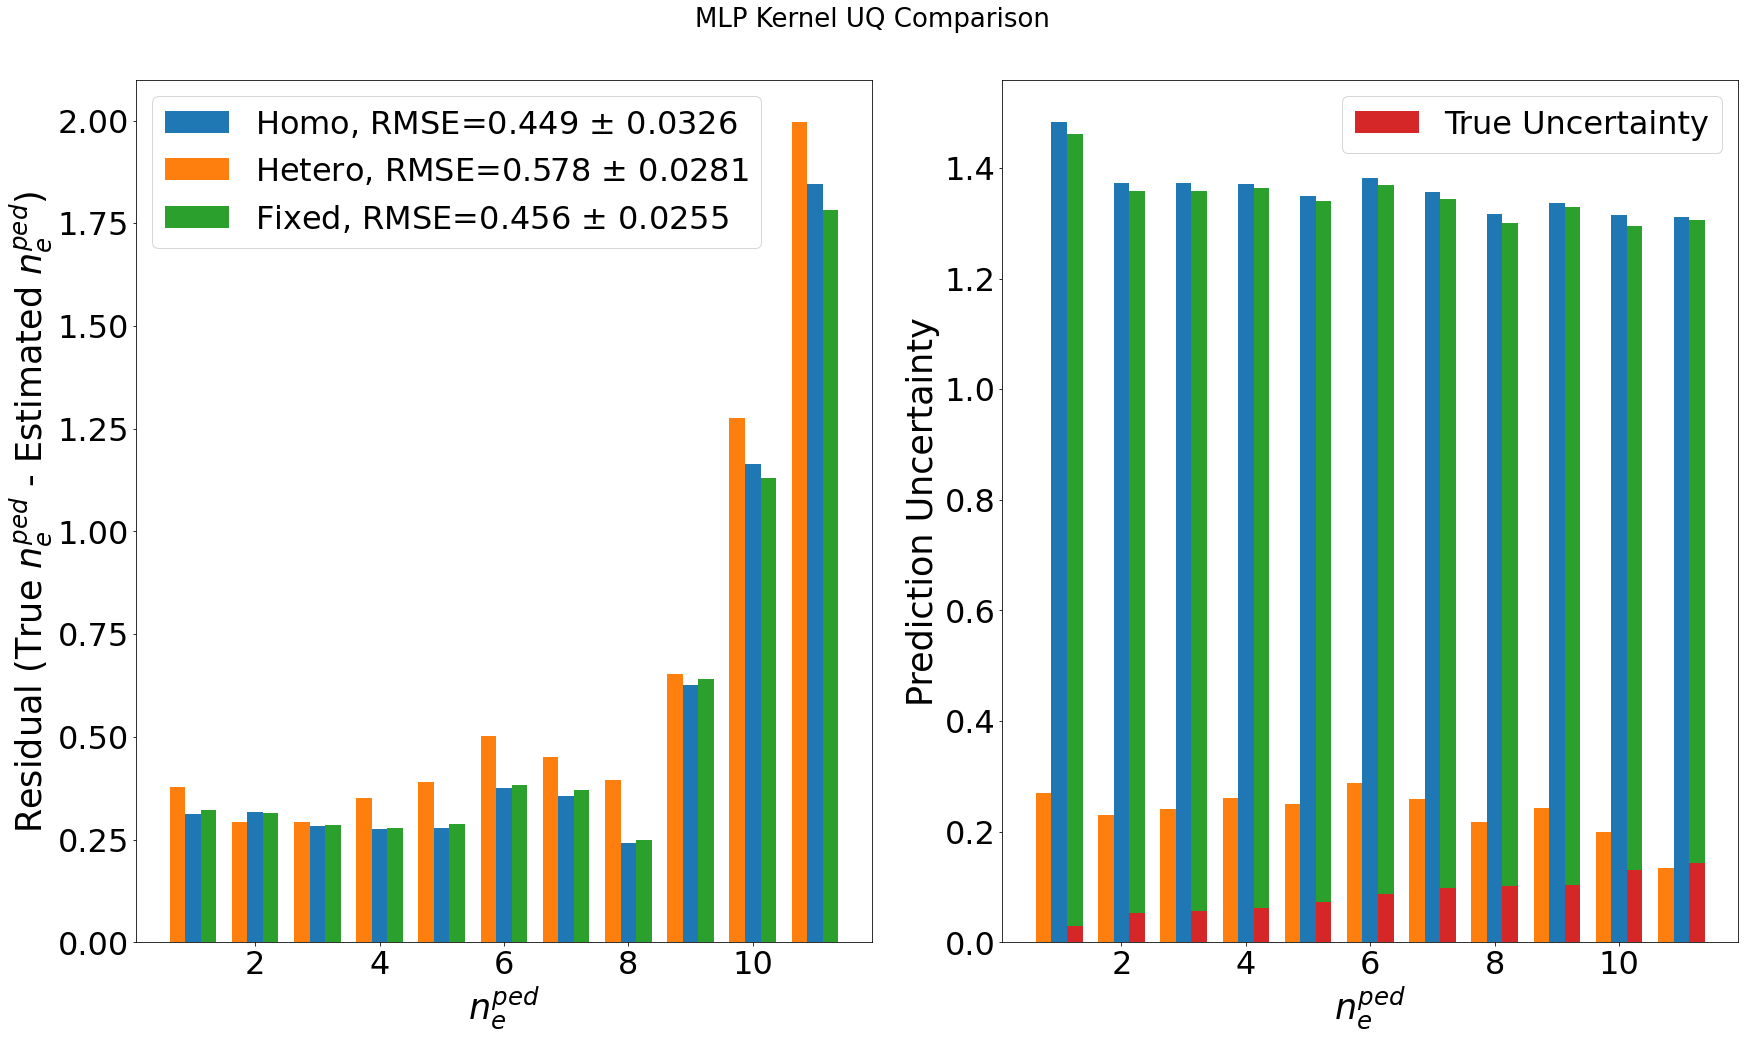
\includegraphics[scale=0.25]{./src/MLP_uq_compare}
		\caption{Three different methods of uncertainty quantification are compared for a GP with an MLP kernel. \textbf{Left:} The true values of $n_e^{ped}$ are grouped into 11 equaly sized bins and the distance between the predictions of those values and the true values are caluclated. The residuals are averaged across each bin and compared between the methods. \textbf{Right:} The same binning procedure, but with averaging the prediction uncertainties of the same three methods are compared.}
	\label{fig:MLP_UQ}
\end{figure}
\begin{comment}
\begin{figure}\centering
		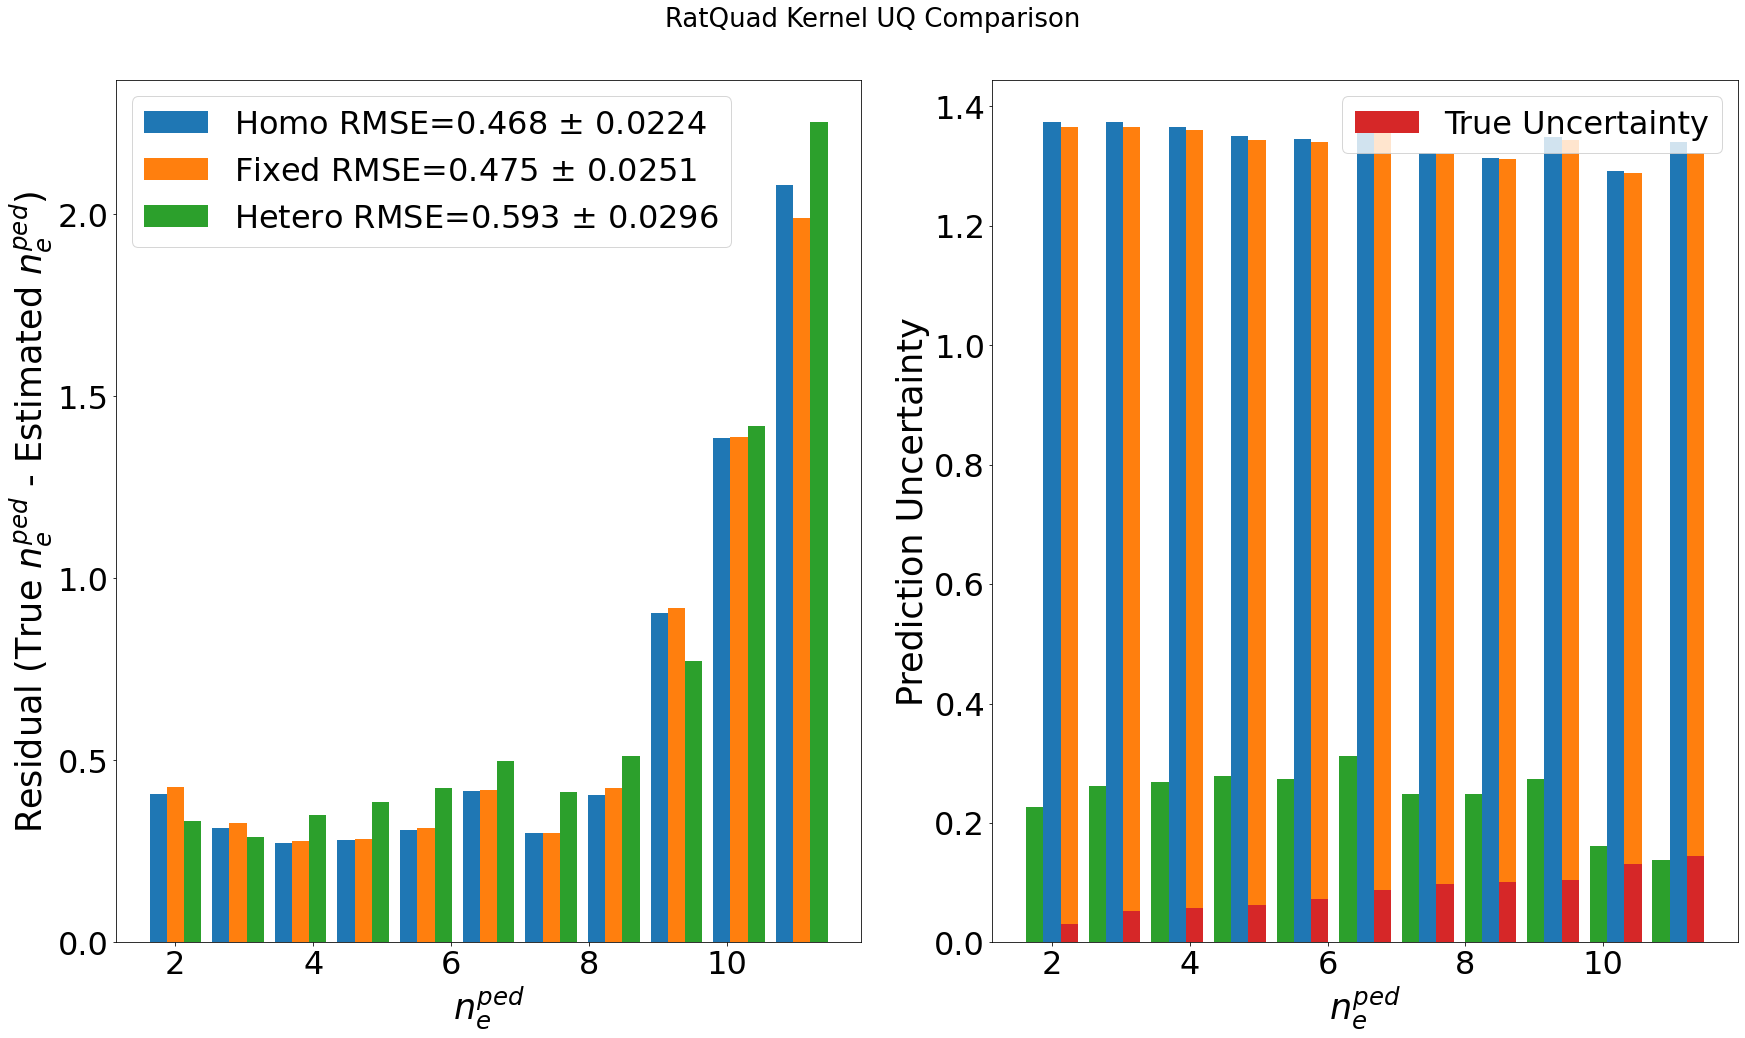
\includegraphics[scale=0.28]{./src/RQ_uq_compare}
		\caption{The same procedure from Figure \ref{fig:MLP_UQ} is applied, just with the Rational Quadratic Kernel instead of MLP.}
	\label{fig:RQ_UQ}
\end{figure}
\end{comment}

\begin{wrapfigure}{r}{0.45\linewidth}
	\caption{}	
	\centering
	\vspace{-14pt}
	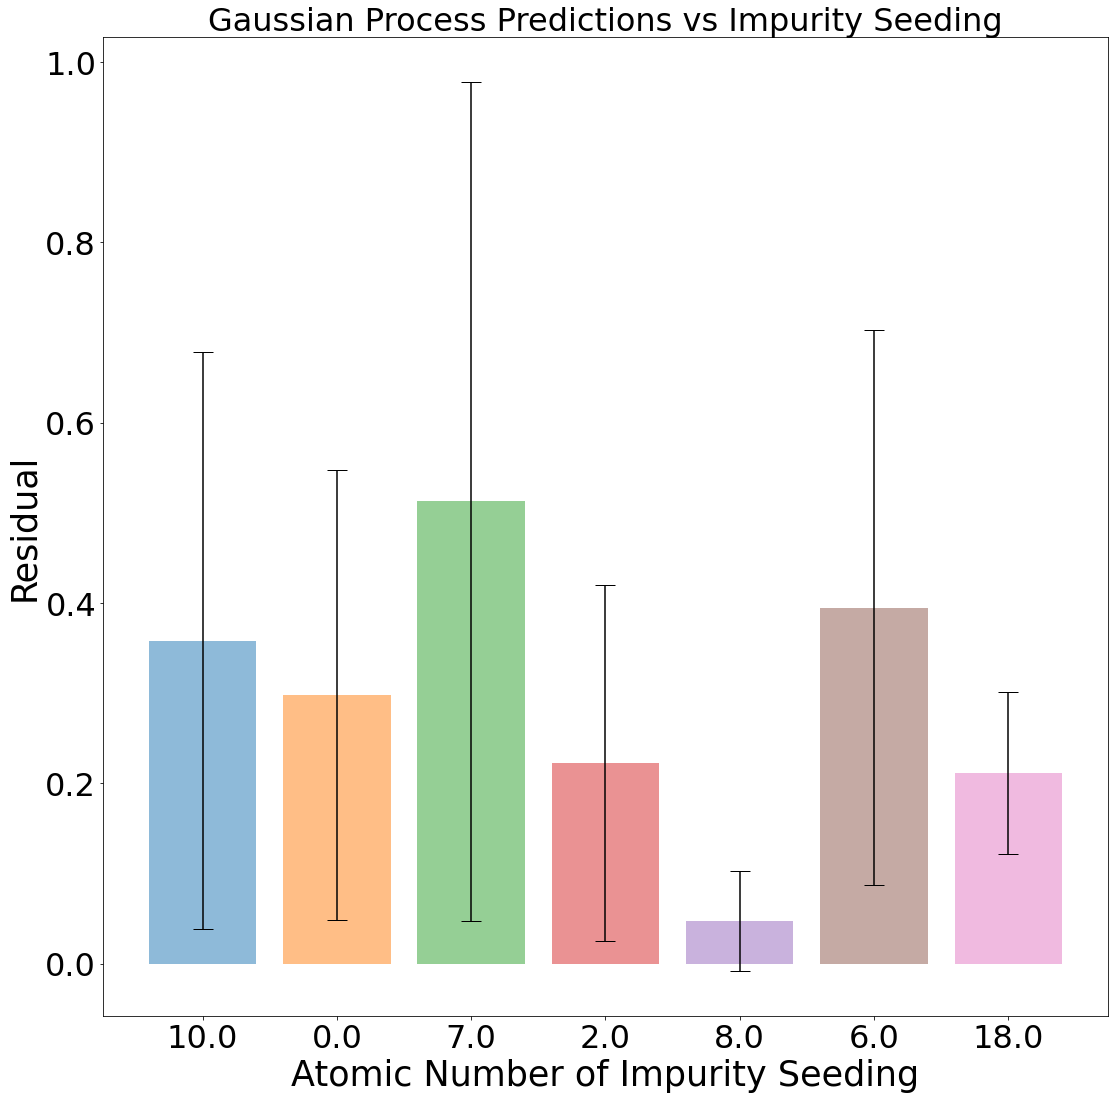
\includegraphics[scale=0.2]{./src/GP_preds_impurity}
	\vspace{-20pt}
	\label{fig:GP_impure}
\end{wrapfigure}
We also compare how the GPs predict on each type of impurity as seen in Figure \ref{fig:GP_impure}. It is well known that Nitrogen (7.0) and Carbon (6.0) play a large roll in the pedestal, and therefore models could in general have the most trouble in predicting these quantities [\textcolor{blue}{SOURCE}]. On the other hand, Neon (10.0) and Argon (18.0) also play a roll on the pedestal (although for different reasons than Nitrogen and Carbon), yet the GPs are able to predict more accurately on those. Nearly three-quarters of the entries in the filtered dataset are unseeded (0.0), and of the remaining third, about 80 percent have Neon seeding, and even fewer of the rest (for example only 3 entries have Argon or Oxygen (8.0) seeding). Even with the equally few amount of entries for both Carbon, Nitrogen, Argon and Neon, the GP models are still able extrapolate the relations of Argon and Neon better than the entries with Carbon and Nitrogen. This suggests that still there exist pedestal dependences on Carbon and Nitrogen seeding that current GP models can not extrapolate.


\subsection{Random Forests}
To deterimine the optimal size (number of decision trees) of an RF and ERT, the out-of-bag error is measured. Additionaly, the optimal number of features to sample in creating each node within each tree can be determined using the OOB, and the results are plotted in Figure \ref{fig:RF_exp}. We see that after 254 decision trees in the RF, the OOB error does not improve, i.e., the forest reaches its maximum generalization capability at 254 decision trees. Furthermore, the optimal number of features to sample is 5. This is completely different for what occurs with the ERTs, where the optimal number of features to sample is 12 (all), and the number of trees is 142. The larger number of features sampled by the ERT compared to the RF is most likely because of the random splitting of nodes that ERTs make use of in creating their trees, such that they need to make use of all the features in order to generalize better, whereas the RF aims to minimize the MSE with their splits, thus not requiring all the inputs for an optimal split. For both models, overfitting begins to occur as more trees are added past the minimum OOB, and although the RMSE may improve, the generalizibility does not.

\begin{figure}
	\begin{subfigure}{0.48\linewidth}
		\centering
		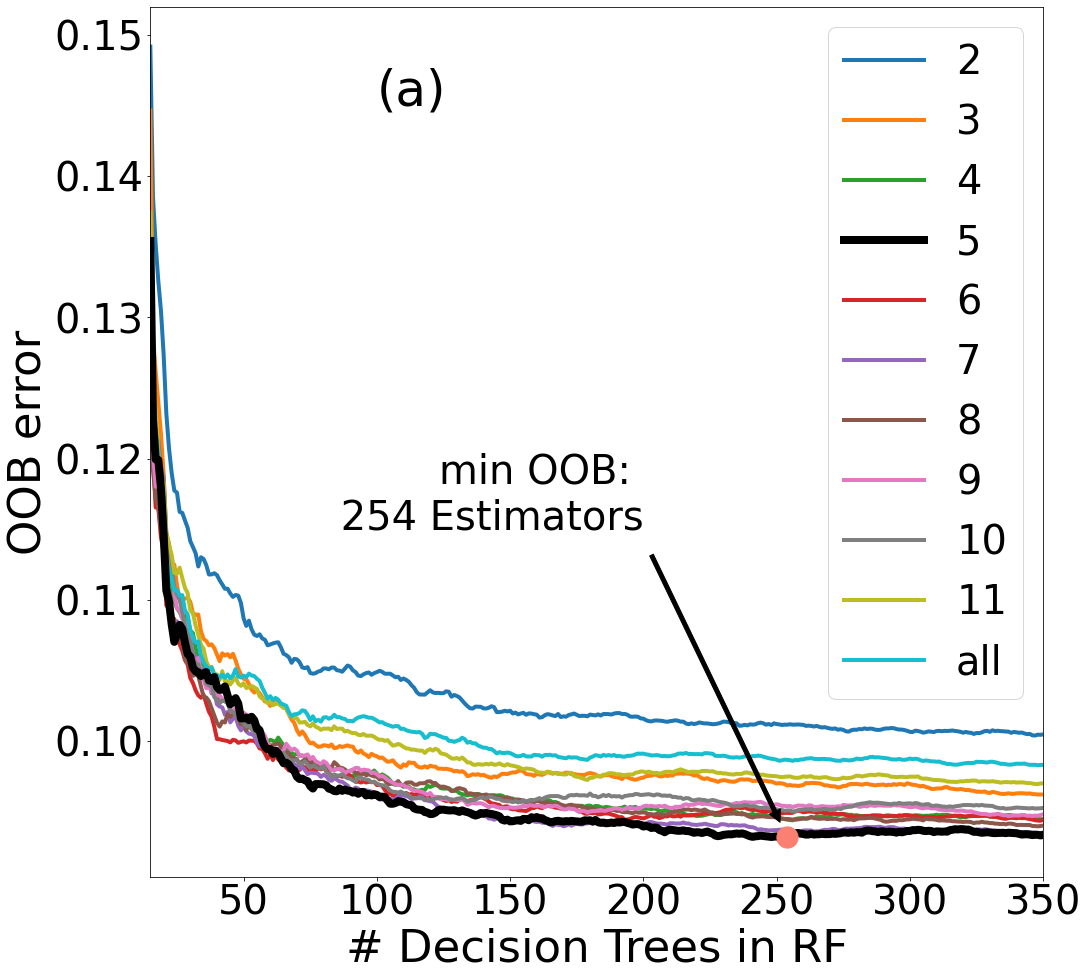
\includegraphics[scale=0.2]{./src/RF_oob_error}
	\end{subfigure}
	\begin{subfigure}{0.5\linewidth}
		\centering
		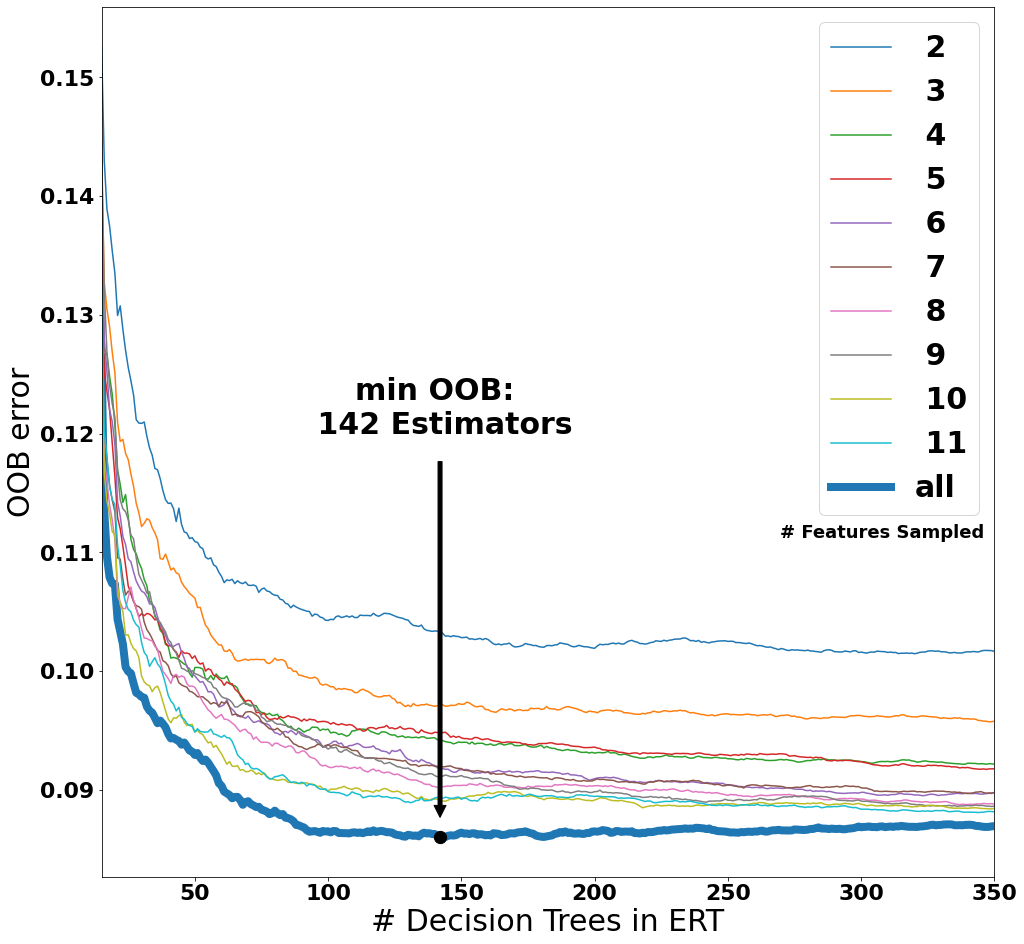
\includegraphics[scale=0.2]{./src/ERT_oob_error}
	\end{subfigure}
	\caption{OOB error vs number of decision trees of \textbf{Left:} Random Forests \textbf{Right:} Extreme Random Trees. No cross validation is necessary for this procedure, since the process of bagging inherently prevents all trees from seeing the same data. The colored lines correspond to different RFs and ERTs which vary by the amount of features to sample when splitting a node.}
	\label{fig:RF_exp}
\end{figure}

Plotted in Figure \ref{fig:RF_Preds} are the resulting predictions from the optimal RFs and ERTs (determined from OOB above), and the uncertainties in the predictions ascertained from the standard deviation between each of the decision tree within the ensemble.
It is clear that the individual predictors in the random forest do not vary as much as that of the homoscedastic/fixed Gaussian Process models. 
Additionally, the uncertainties are able to generally be around equal to that of the residual for the corresponding bin. This is good, as the model is able to more or less provide an uncertainty that covers its residual. This does not hold for $n_e^{ped} \geq 10.0$, but it is certainly within the ballpark. 

\begin{wrapfigure}{r}{0.5\textwidth}
		\centering
		\vspace{-20pt}
		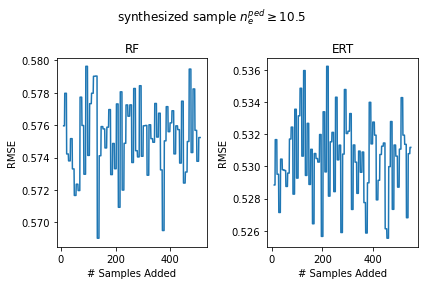
\includegraphics[width=\linewidth, keepaspectratio=true, trim=0 0 0 30, clip]{./src/ERT_vs_RF_meta_modeling}
		\vspace{-22pt}
		\caption{Effect of Meta Modeling in RF and ERTs. The \# of synthesized samples added into dataset is plotted against the resulting RMSE of an RF/ERT that is fit with the additional number of synthesized samples added into its training dataset.}
		\label{fig:RF_meta_model}
\end{wrapfigure}
Metamodeling had generally no effect on RFs and ERTs, as seen in Figure~\ref{fig:RF_meta_model}.
For the RF, splits in the nodes of the decision trees are made only when the RMSE of the prediction decreases, whereas for the ERT the split is randomly selected from the distribution of parameters within input space.
Although only up to 500 meta model samples are visualised in Figure~\ref{fig:RF_meta_model}, the sporatic bouncing of the RMSE between 0.57 and 0.58 repeats for when even 2000 synthesized entries are added!
This suggests that in order to minimize the MSE of predictions across the entire dataset, RFs and ERTs ignore the additional entries and in  conclusion that meta-modeling has little to no effect on ERTs and RFs.

\begin{figure}[t]
		\centering
		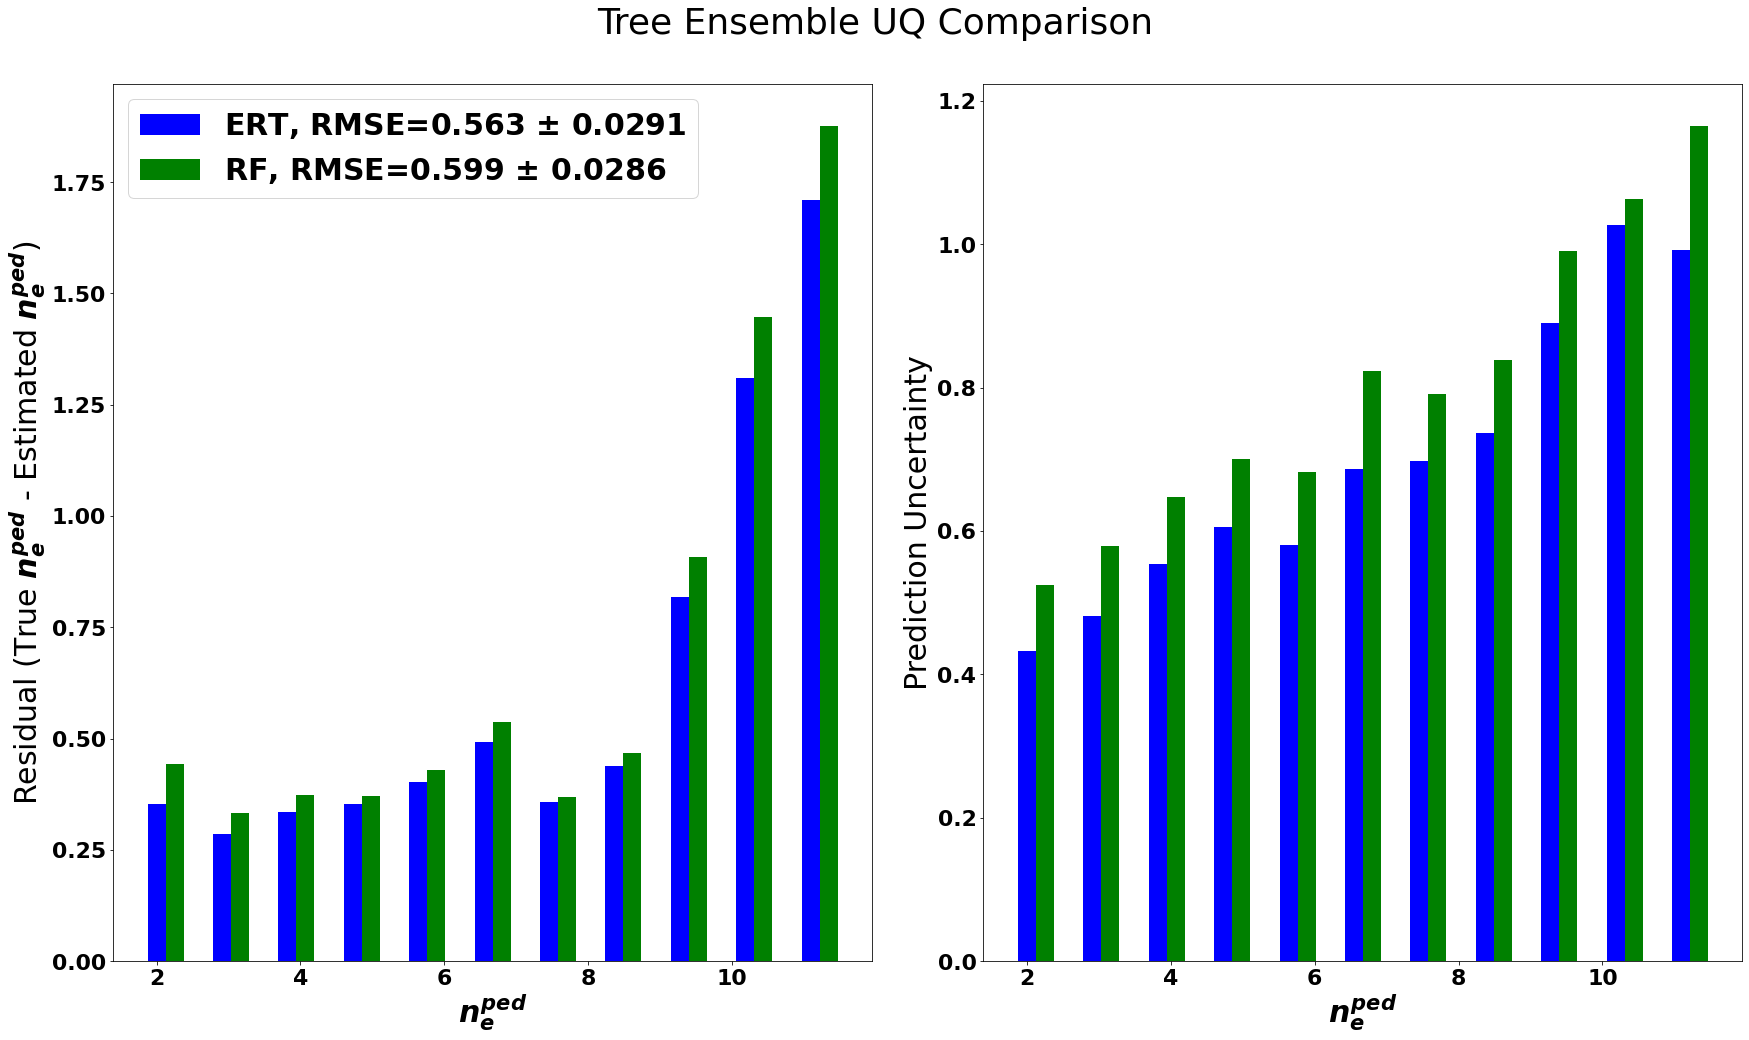
\includegraphics[scale=0.25]{./src/Tree_UQ}
		\caption{Comparison of predictions and uncertainties between Random Forests (green) and Extreme Random Trees (blue). \textbf{Left:} The residual between predictions and the true values,\textbf{Right:} The prediction uncertainties on the same bins of the residuals. }
	\label{fig:RF_Preds}
\end{figure}
\subsection{Artificial Neural Networks}

\begin{wrapfigure}{r}{0.5\linewidth}
	\centering
	\vspace{-45pt}
	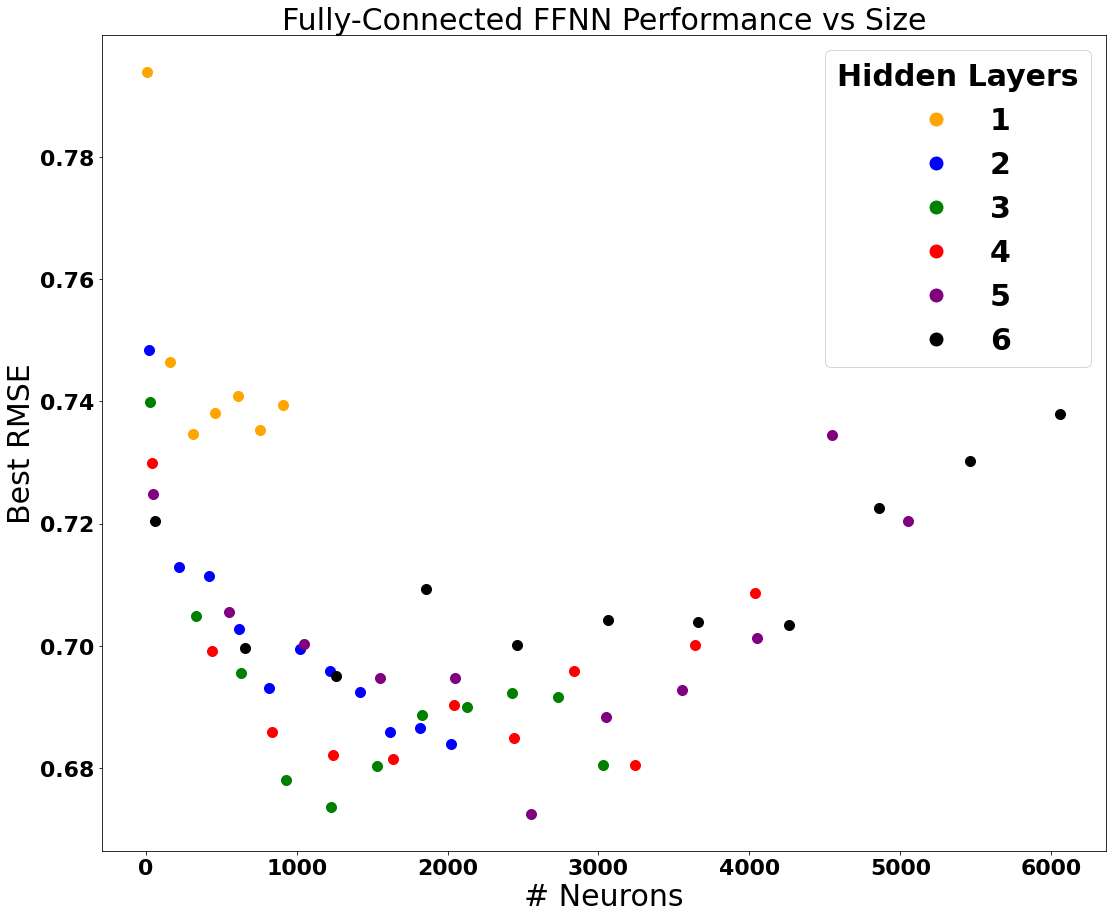
\includegraphics[scale=0.2]{./src/ANN_performace_size}
	\caption{}
	\vspace{-11pt}
	\label{fig:ANN_dim}
\end{wrapfigure}
From Figure \ref{fig:ANN_dim}, we see that shallow ANNs ($3-5$ hidden layers)  perform the best, therefore the hyperparameter optimization process is focused on these networks. Since the main engineering parameters vary in magnitude (scalar value of $P_{TOT}$ is much greater than that of $q_{95}$), each parameter is scaled such that it has a mean of 0 and standard deviation of 1. Throughout the hyperparameter optimization process, each model was trained and tested using the repeated cross-fold validation method, with 5 folds and 5 repeats, and the average RMSE of predictions on the left out sets is the overall performance of the ANN. The first hyperparameters to be optimized are the learning rate and mini-batch size, and using random search, the optimal MBS and LR were found to be 396 and 0.004 respectively. Considering the dataset is around 2000 entries, the mini-batch size is relatively large, and the learning rate could be considered very small for such a large mini-batch size. However, since each training epoch, the data is randomly shuffled, it is possible that the training samples in each batch 'compete' with eachothers gradient. For example, the training samples of $n_e^{ped} \geq 9.5$ pull the model weights in an opposite direction than that $n_e^{ped} \leq 9.5$. The gradient updates applied by the learning rate for this mini-batch size seemed to balance the effect of the training samples, thus resulting in the best training/testing performance. 

Then, via grid search (across all available activation layers offered by Pytorch), the optimal activation function was deterimend to be ELU (Exponential Linear Unit), a close cousin to the well known ReLU (Rectefied Linear Unit) [\textcolor{blue}{SOURCE}]. Both are ridge functions that act on a linear combination of the input variables, but since they are applied element-wise (for each node in each layer), they are non-linear. Since the above tools like GPs and RFs are non-linear models, it makes sense that a non-linear activation function performs the best. 

Using these hyperparameters, models of varying sizes of hidden layers were fit, and as seen in Figure \ref{fig:ANN_dim}, the initial ansatz of optimal hidden layers was determined to be either 3, 4 or 5, with between 1000-2000 total nodes (split between each of the hidden layers). This criteria was used as a space for further architecture search via random search.
The optimal sizes of each layer for 3, 4, and 5 hidden layer networks is listed below. 
\begin{itemize}
	\item \textbf{3 Hidden Layers}: 483, 415, 254
	\item \textbf{4 Hidden Layers}: 636, 537, 295, 261
	\item \textbf{5 Hidden Layers}: 390, 484, 678, 290, 284
\end{itemize} 
Of the networks listed above, the one with 4 hidden layers performed the best, with an optimal RMSE of $0.6596 \pm 0.023$. 
It was generally seen that shallow networks ($\leq 4$ hidden layers) with steadily decreasing layer size performed the best, whereas the larger networks performed best with this 'bell' shaped sizes, as seen in the 5 hidden layer network above. 
There could very well be better sizes out there, but the general idea of large first hidden layer followed by steadily decreasing layer sizes performs the best.

At the end, the best performing 3 layer ANN was used to make an ensemble, with each ANN within having different initial weights, and the prediction and uncertainty was compared across varying ensemble sizes. The ensemble was fitted in the same cross-validation format, with 5 folds and 5 repeats. We see in Figure \ref{fig:ANN_UQ} that as the ensemble size grows, there is a slight decrease in RMSE and thus improved prediction quality. However, this comes with the cost of higher prediction uncertainty, where the uncertainty in the ensemble with 15 ANNs has nearly double the uncertainty for that of 5 ANNs. Although the prediction uncertainty covers the spread, it does so by a margin that resembles the GPs, however they do increase as we reach higher pedestal densities unlike that of the GPs. 

Meta modeling as an additional form of UQ did seem to improve predictions for high $n_e^{ped}$, while sacrificing the overall performance.
This was unique for the ANNs, as all other usages of meta-modeling for other ML tools either did not affect the model or had only adverse effects to performance.
\begin{figure}
	\centering
	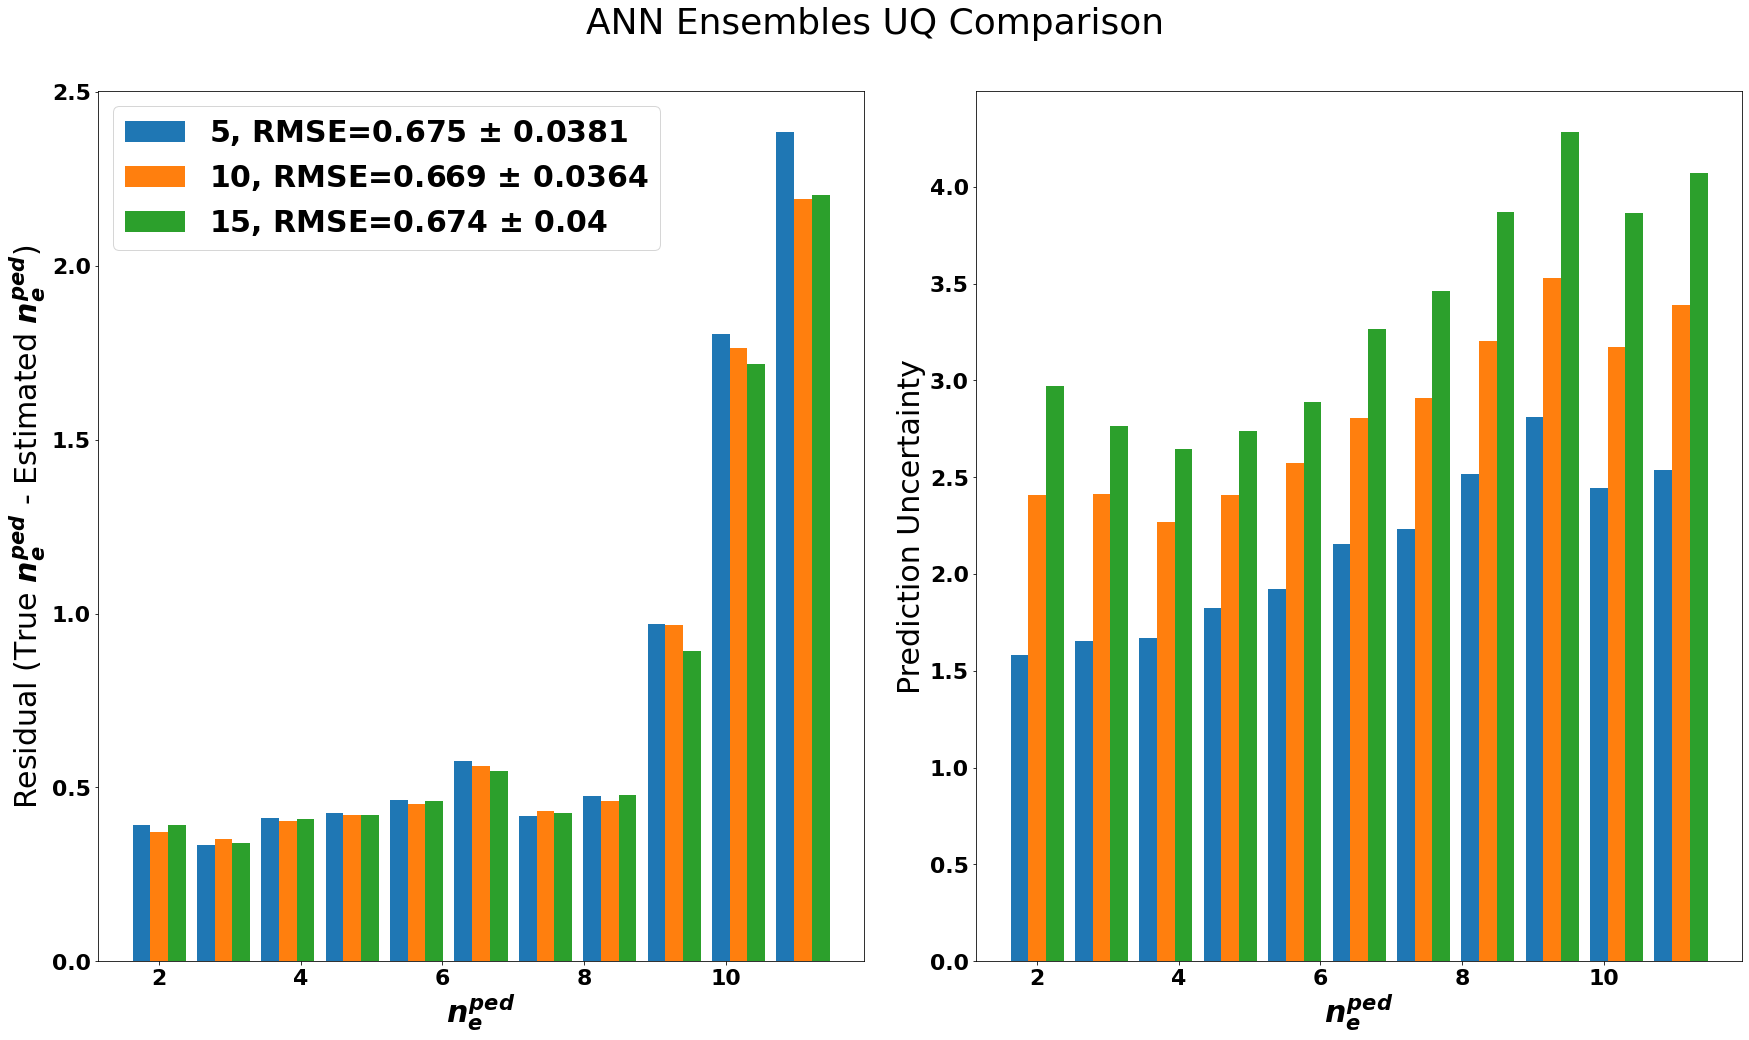
\includegraphics[scale=0.25]{./src/ANN_ensemble_comp}
	\caption{A three layer feed foward fully connected ANN with layer sizes 483, 415, 254 was transformed into ensembles of sizes 5 (blue), 10 (orange, 15 (green). }
	\label{fig:ANN_UQ}
\end{figure}
\begin{comment}
\begin{figure}
	\begin{subfigure}{0.49\linewidth}
		\centering 
		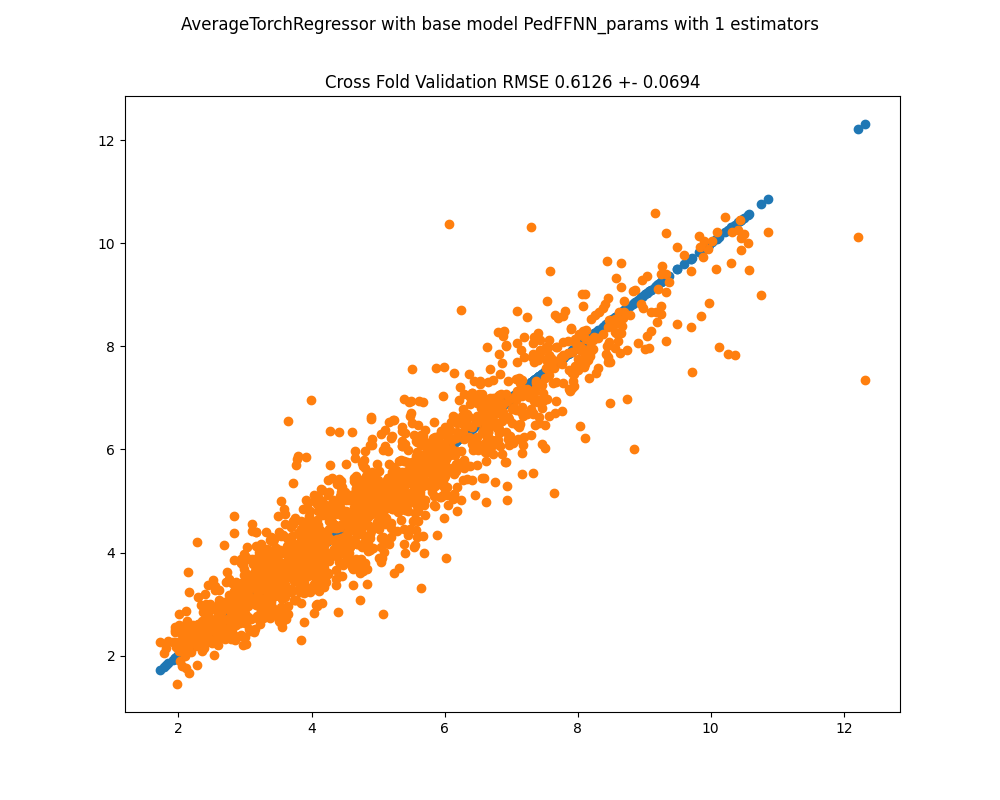
\includegraphics[scale=0.3]{./src/ANN_1}
		\caption{}
		\label{subfig:ann_1}
	\end{subfigure}
	\begin{subfigure}{0.5\linewidth}
		\centering
		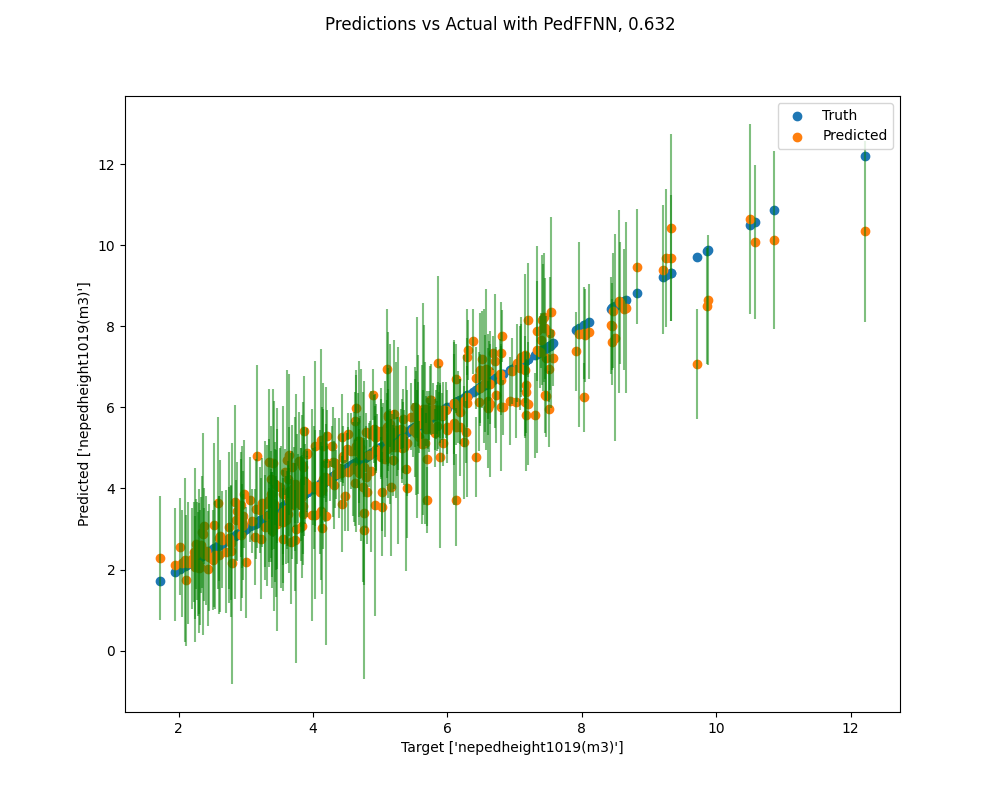
\includegraphics[scale=0.3]{./src/ENSEMBLE_5}
		\caption{}
		\label{subfig:ensemble}
	\end{subfigure}
\end{figure}
\end{comment}
\subsection{What didn't work}
Many different machine learning models not listed in the above analyses were initially tested, but due to their underperformance compared to RFs/GPs/ANNs, they were abandoned before delving deeper into the others. For example, Nearest neighbours methods like K-nn and R-nn were tested and abandoned. Radius neighbours especially so, which although they could overfit extremely well with sufficiently small radius, they can not generalize for data entries which they are not fitted with, most often providing no prediction. Support vector machines (SVMs) were tested, but due to the difficulties of deriving the prediction uncertainty and general underperformace, they were dropped. Additionally, SVMs work well when there is a clear seperation between regression points, but as we have seen, for $n_e^{ped} \geq 9$ there is no clear cut discrepncies, so SVMs offer little to no utility. Additionally, it is difficult to obtain uncertainties in predictions when using neighborhood methods and SVMs, and one of the goals of this thesis was to analyse models that could provide uncertainties. Other ensemble methods like AdaBoost showed to perform equally or slightly worse than RFs and ERTs, but some scope was needed in this thesis, so they were ultimately dropped from analysis. The combination of multiple model types into an ensemble (e.g. voting ensemble of ERT, RF and GPs) proved only slightly beneificial, and may be looked into futher in future research. 
\section{Conclusion and Outlook}
\begin{table}
	\begin{center}
		\begin{tabular}{| c | c | c |}
		\hline
		Model & RMSE & MAE \\
		\hline
		Scaling Law & $0.9203 \pm 0.63$ & TBD \\
		\hline
		Linear & $0.8166 \pm 0.0605 $ & $0.5956 \pm 0.0379$ \\
		GP & $0.4566 \pm  0.0217$ &  $0.3395 \pm 0.01383$\\
		RF & $0.5938 \pm 0.0352$ & $0.4225 \pm 0.0191$ \\
		ERT &$0.5623 \pm 0.0368 $ & $0.3927 \pm 0.0199$ \\
		ANN & $0.6126 \pm 0.0694$ & TBD \\
		\hline
		\end{tabular}
		\caption{The optimal relevant hyperparameters are chose for each model type, and the best RMSE and MAE are caulculated by averaging the results across each fold and repeat of the repeated cross-validation method. Uncertainty in the calculated RMSE and MAE is derived from the  standard deviation of the RMSE across each fold.}
		\label{tab:performance_models}
	\end{center}
\end{table}
It is clear that through the use of non-linear machine learning models, there can be major improvements towards accurately predicting the pedestal density height while only using main engineering parameters.

The models analysed are ranked via their respective performance on unseen data through the use of cross validation, which is given in Table \ref{tab:performance_models}.
It is hard to point to a clear winner among the non-parameteric/linear models, as they all score relatively close to eachother, but it is easy to see that all ML tool analysed outpreform the scaling law. Strictly speaking, the homoscedastic Gaussian Process model with an MLP kernel achieved the lowest RMSE and MAE. All models could predict well on pedestal densities less than 9.5, however they also all struggled on densities higher than that. Future work would include analysis on how splitting the data into different subsets (e.g., two subsets, one with low density, one with high density) and fitting models on the independent subsets affects predictions. This could be extended not just for splitting high and low density, but also for example low and high $q_{95}$. The non-linear models performed worse on Carbon and Nitrogen seeded entries than they did for other impurity seedings, therefore future work would include further independent analysis into why that happens.  

For each model, the prediction uncertainty was ascertained. The prediction uncertainty for Random Forests, Extreme Random Trees, aptly covered the residuals of their predictions without being 'overly cautious', while the homoscedastic and fixed kernel GPs generally held relative constant and high uncertainties for each prediction. We were able to utelize the measurement uncertainties of $n_e^{ped}$ in the JET pedestal database by propogating them into a heteroscedastic Gaussian Process model, and were ultimately able to (roughly) map the latent uncertainty space. This could prove useful should these machine learning models every be used as surragate models in simulations. Future work on uncertainty quantification would likely include using the main engineering parameters, for example using a fixed kernel like was done for $n_e^{ped}$. 

The effect of meta-modeling was limited to RFs and ERTs, but from this we were able to ascertain that there is no effect on these types of models. Future work would include using meta-modeling on GPs and ANNs.  



\begin{comment}

\section{Results2}\label{sec:results_2}
The list of initial control parameters is the same for every model is rewritten below: 
\begin{itemize}
	\item $Z_{eff}, I_p, B_T, a, \delta, M_{eff}, P_{NBI}, P_{ICHR}, P_{TOT}, q_{95}, \Gamma, H, \Gamma_{SD}$.
\end{itemize}
The correlation matrix and Spearman rank-order correlation plots are found in Figures \ref{fig:corrshit}

\begin{figure}
	\centering
	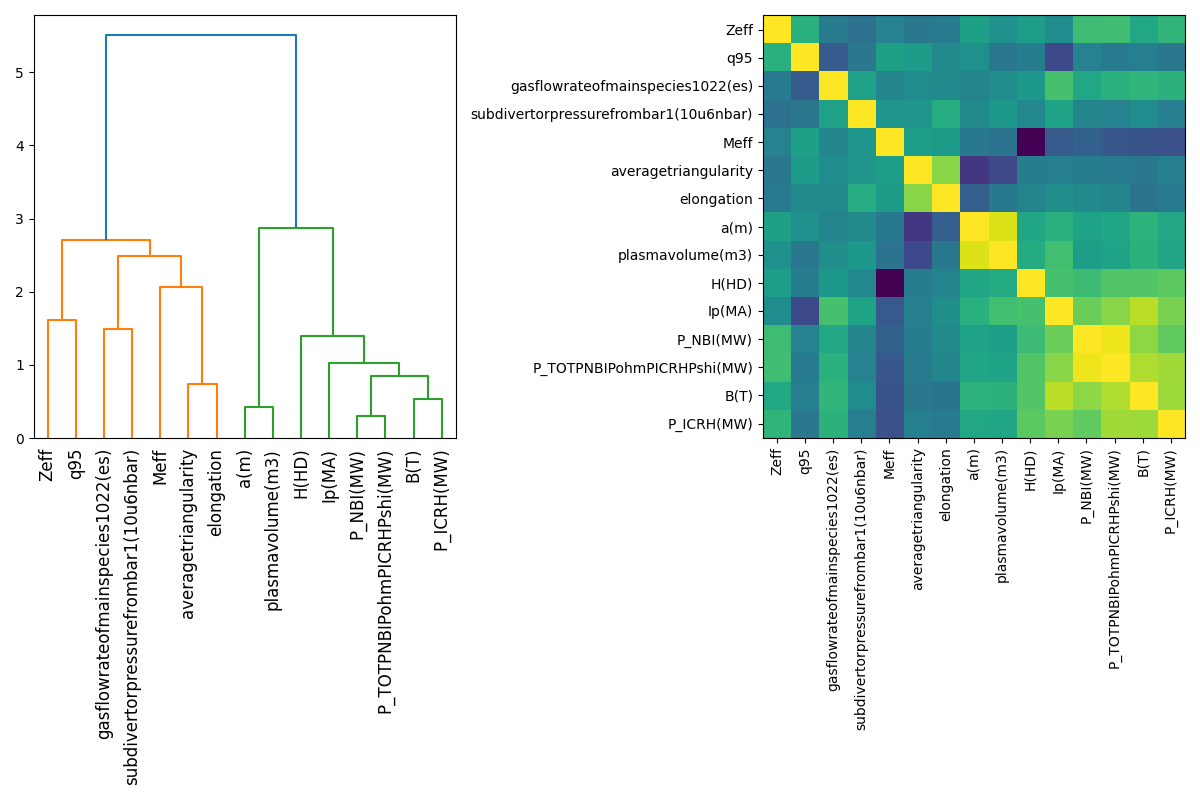
\includegraphics[width=0.9\linewidth, keepaspectratio=true]{./src/correlation_shit}
	\caption{LHS: the Spearman rank-order correlation plot.  RHS: the correlation matrix for the initial control parameters}
	\label{fig:corrshit}
\end{figure}
\subsection{Linear Regression}
\begin{figure}[t!p]
	\begin{subfigure}[b]{0.45\linewidth}
		\centering
		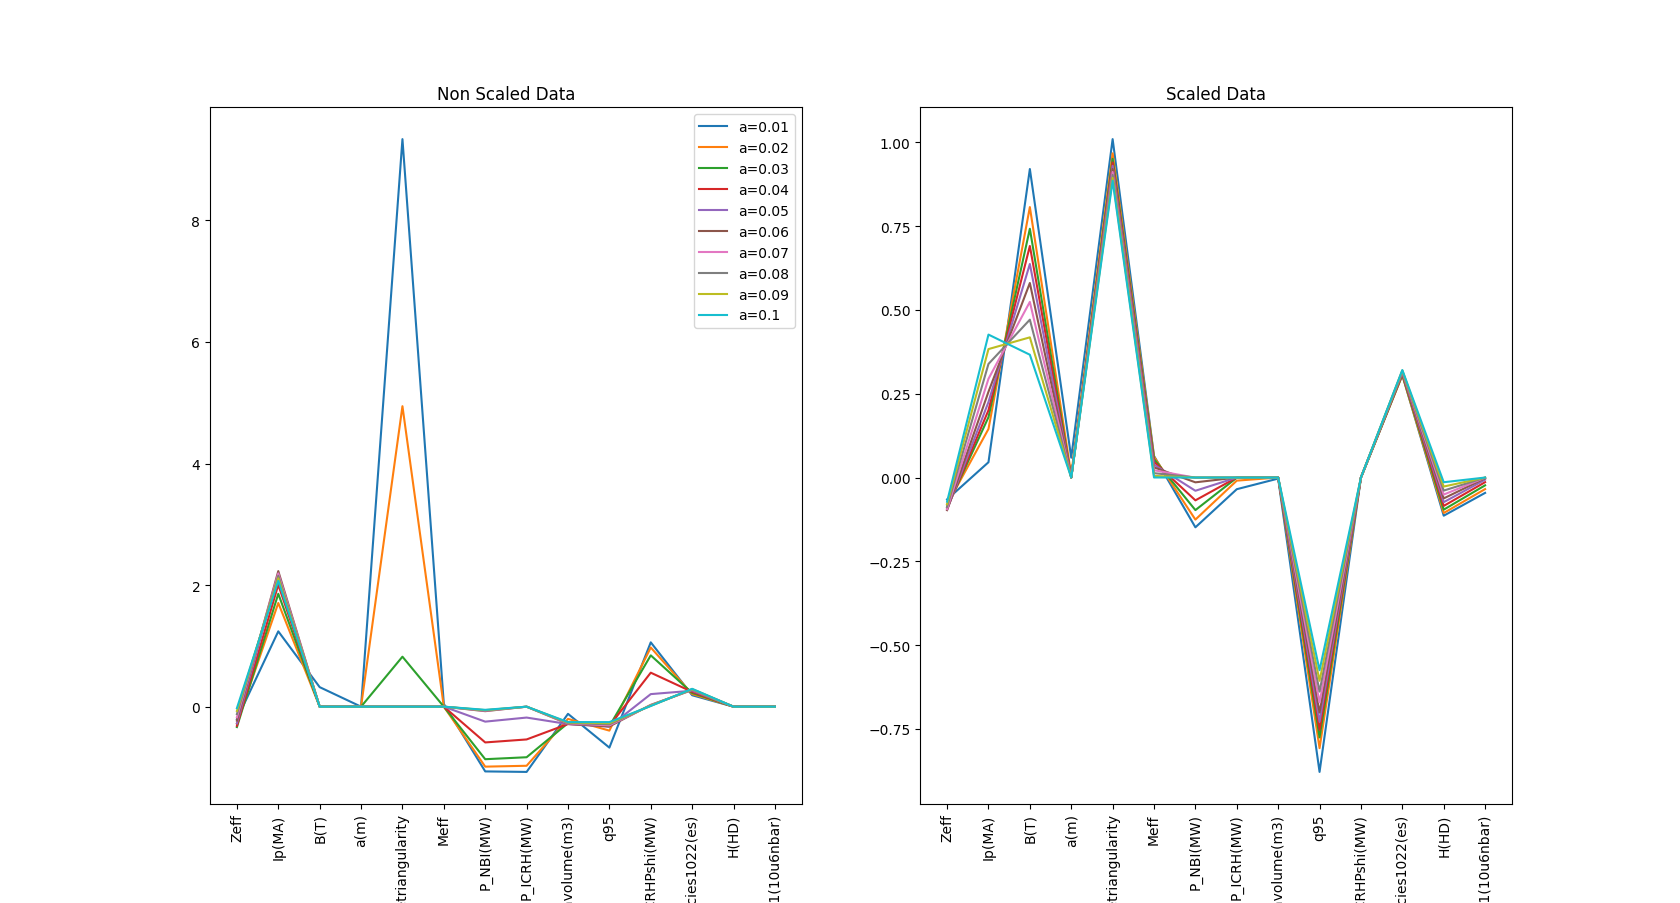
\includegraphics[width=0.9\linewidth, keepaspectratio=true]{./src/Lasso_feature_selection}
		\caption{}
		\label{subfig:lasso_FS}
	\end{subfigure}
	\begin{subfigure}[b]{0.5\linewidth}
		\centering 
		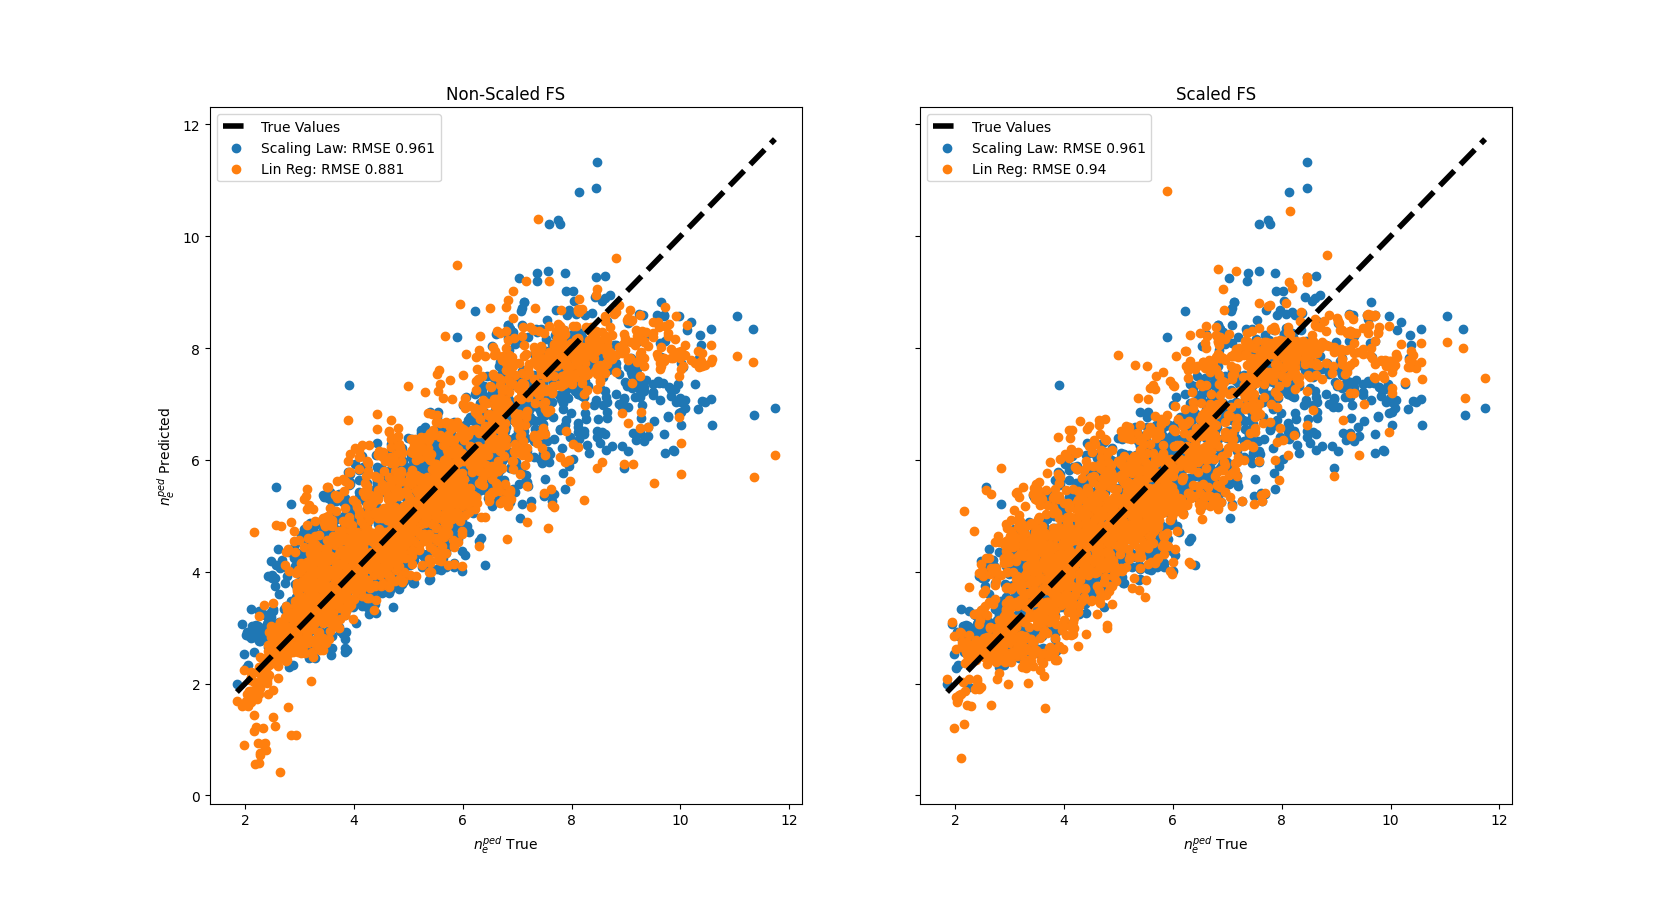
\includegraphics[width=0.9\linewidth, keepaspectratio=true]{./src/regressor_using_Lasso_feature_selection}
		\caption{}
		\label{subfig:reg_FS}
	\end{subfigure}
	\caption{Feature selection (a) and prediction quality (b) for linear regression}
	\label{fig:lin_exp}
\end{figure}
I compare how the Lasso method of feature selection works with two different version of the dataset: the 'as is' data, the data scaled such that each feature has a mean of 0 and spread of 1.
It is important to note that the prediction quality of the Lasso models is not entirely important, as $\lambda = 0$ would yield the best results, but would not indicate importance of features at all.  
The results of the LASSO method for various values of $\lambda$ on the two versions of the dataset, non scaled and scaled, are plotted in \ref{subfig:lasso_FS}. 
For the nonscaled data, by averaging over all the differnt values of $\lambda$, the following features were deemed most important: $I_p, \delta, P_{NBI}, P_{ICRH}, V_P, P_{TOT}, q_{95}, \Gamma$.
For the scaled data, the following features were deemed important: $I_p, \delta, P_{NBI}, B_T, q_95, \Gamma, H$. 
Interestingly enough, both the scaled and nonscaled data deemed the following features as not relevant: $B_T, Z_{eff}, M_{eff}, a, \Gamma_{SD}$, where $B_T$ seems most suprising to me. 
Then, aggregating new feature spaces using the two sets of generated features, a linear regressor (using OLS and without regularization) is fit and compared against the scaling law in Figure~\ref{subfig:reg_FS}. Both the new sets produce regression predictors better than the scaling law, with the regressor trained on the non-scaled fit performing substaintially better than than both. Both do are able to capture higher values of $n_e^{ped}$ better than the scaling law, but slightly struggle on those close to 0. 
Using features determined from the Lasso method on non-scaled data, it seems viable that a new scaling law could be written using the coefficients of a regressor fitted using those features. 
For UQ of linear regression tools, I employ Baysian regression, which transforms the coefficients to distributions, giving the overall uncertainty in the prediction from the spread of each of the weight distributions. 

\subsection{Gaussian Processes}
\begin{figure}
	\begin{subfigure}{0.5\linewidth}
		\centering
		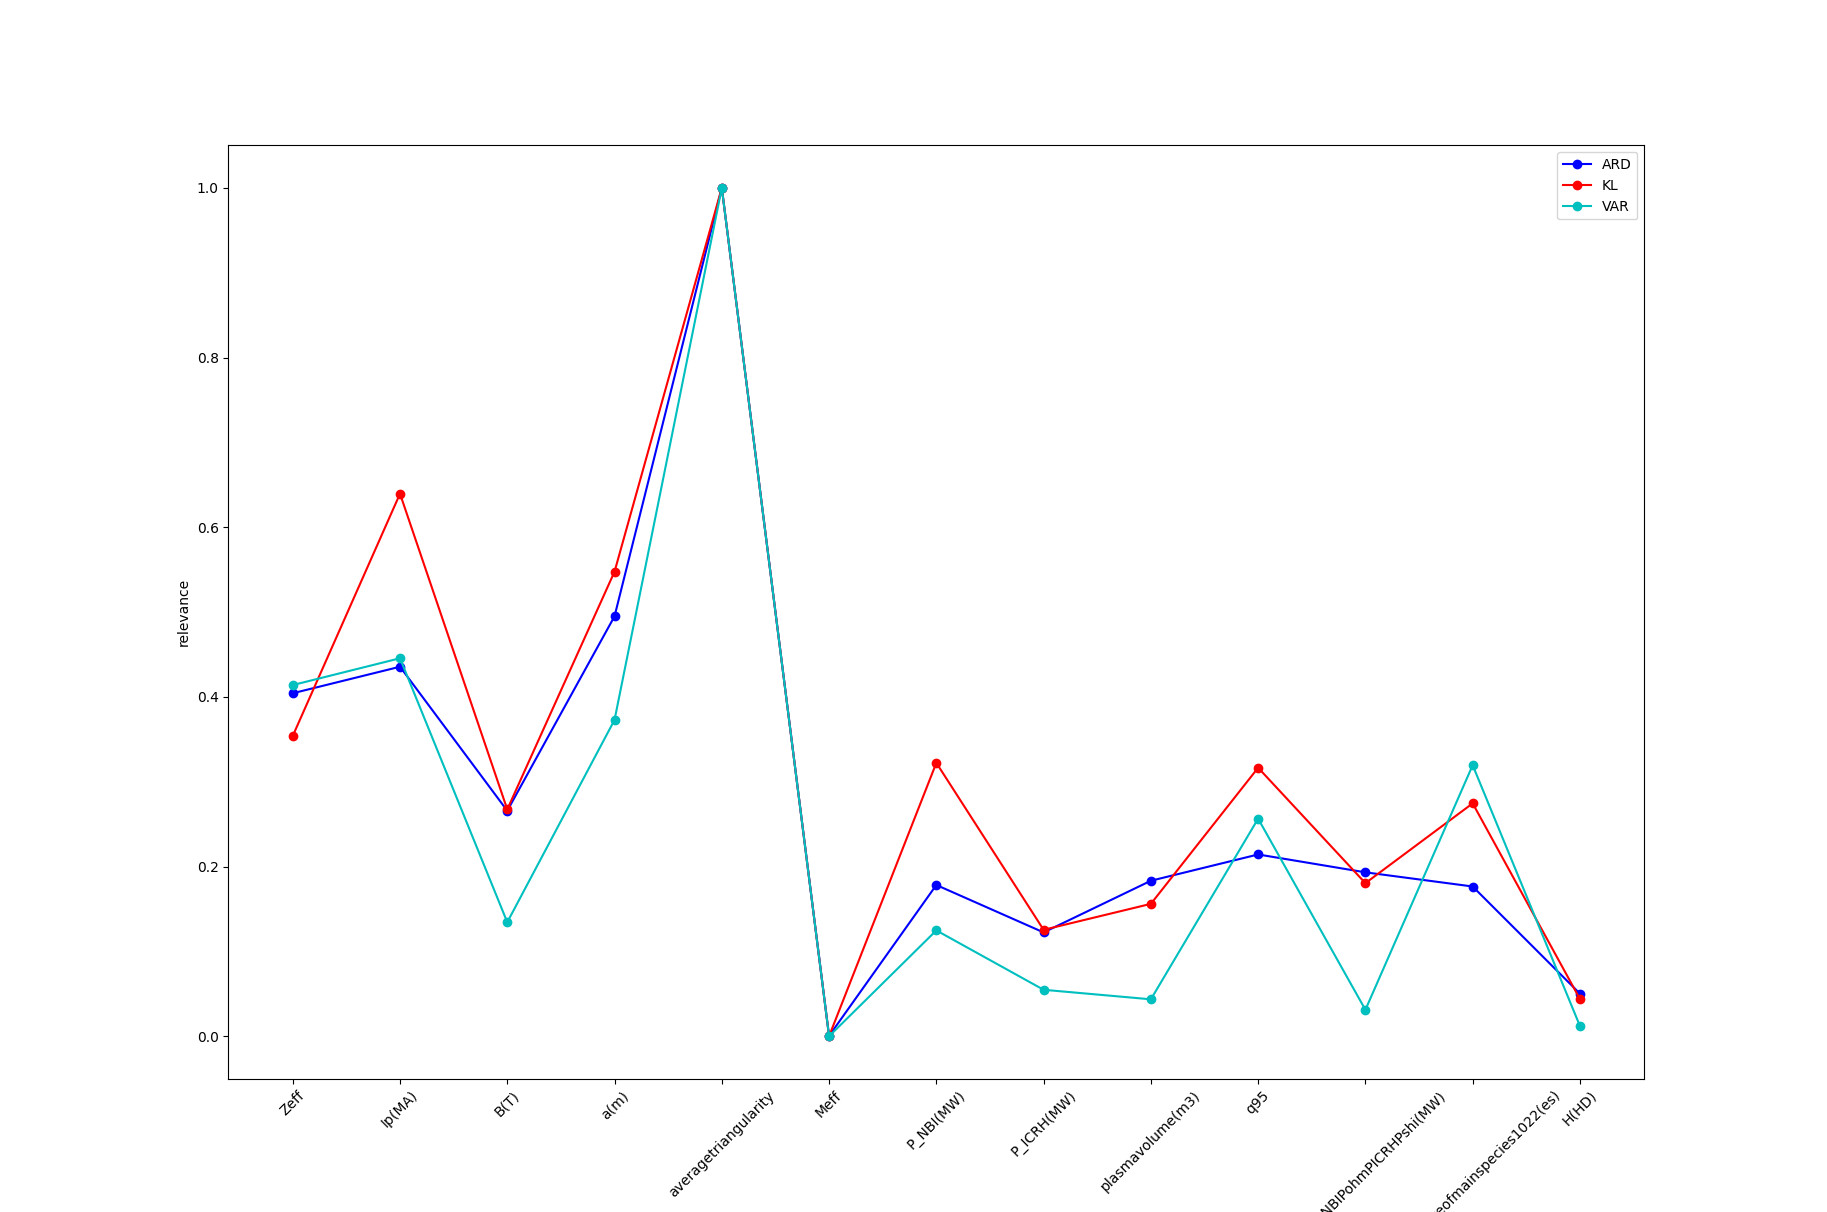
\includegraphics[width=0.9\linewidth, keepaspectratio=true]{./src/ARD_vs_KL_VAR_feature_relevance_final_maybe}
		\caption{}
		\label{subfig:gpfs}
	\end{subfigure}
	\begin{subfigure}{0.5\linewidth}
		\centering
		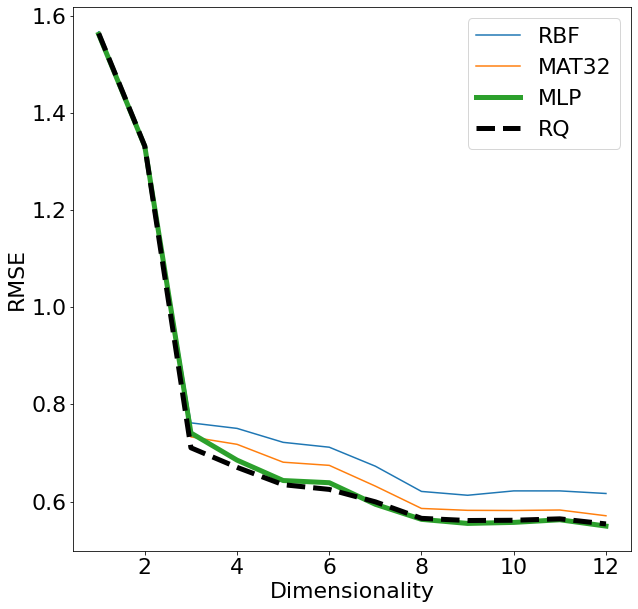
\includegraphics[width=1\linewidth, keepaspectratio=true]{./src/GP_kernels_num_features}
		\caption{}
		\label{subfig:gp_dim}
	\end{subfigure}
	\caption{Feature selection (a) and Prediction quality (b) for Gaussian Processes}
	\label{fig:gp_exp}
\end{figure}
Before testing out ARD, KLD, and VAR, both control features and $n_e^{ped}$ are scaled such that they have mean of 0 and spread of 1. This is necessary for GPs. 
The features can be ranked through the use of ARD, KLD, and VAR, and are listed below in order of importance as plotted in \ref{subfig:gpfs}. 
\begin{itemize}
	\item \textbf{ARD}: $\delta, I_p, Z_{eff}, a, \Gamma, q_{95}, B_T, P_{NBI}, P_{ICRH}, V_P, P_{TOT}, H, M_{eff}$
	\item \textbf{KLD}: $\delta, I_p, a, Z_{eff}, P_{NBI}, q_{95}, B_T, \Gamma, P_{TOT}, V_P, P_{ICRH}, H, M_{eff}$
	\item \textbf{VAR}: $\delta, a, I_p, Z_{eff}, B_T, q_{95}, P_{TOT}, V_P, \Gamma, P_{NBI}, P_{ICRH}, H, M_{eff}$
\end{itemize}
$\Gamma_{SD}$ is not included, as it seemed to play absolutely no benefit in the gaussian process predictions, and would tend to disrupt the feature selection methods when included. 
Although they may rank each feature differently, it is interesting to note that the top 4 features that are relevant to predicting $n_e^{ped}$ are always triangularity, current, minor radius and effective charge. Furthermore, where the lasso disregarded $Z_{eff}, B_T$ and $a$, the GP methods consitently rank these among in addition to the transport in the plasma of the highest of importance. The reason each method consistantly ranks the power parameters among the lowest is because the dependence of $n_e^{ped}$ on power is relatively weak. Just like in the scaling law, 

Following the selection of features, I fit 14 GP models using the KLD order, with the first model using onlly $\delta$ as input, thus dimensionality of 1, followed by the next model using $\delta, I_p$, with dimensionality 2, and so on following the KLD order of importance. The results are plotted against the RMSE of each fitted model while comparing three different kernels in Figure \ref{subfig:gp_dim}. NOTE.TO.AARO: [This plot is not finished, I need to rerun the experiment using the KLD, VAR, and ARD methods and make three plots to compare. Also the dimensionality list is not actually that of KLD but slightly different. So need to particullary rerun KLD ]. From the plot, I deduce that the Rational Quadratic (RQ) kernel outpreforms the Matern kernel, which in turn outpreforms the Radial Basis Function (RBF). For both RQ and Matern, the RMSE does not improve after dimensionality 10, which happens to be $V_P$, thus further confirming the unimportance of $V_P, P_{ICRH}, H, M_{eff}$. The uncertainty lines atttached to each point are from the cross validation methods used. 

\subsection{Random Forests and Extreme Random Trees}
\begin{figure}
	\begin{subfigure}{0.5\linewidth}
		\centering 
		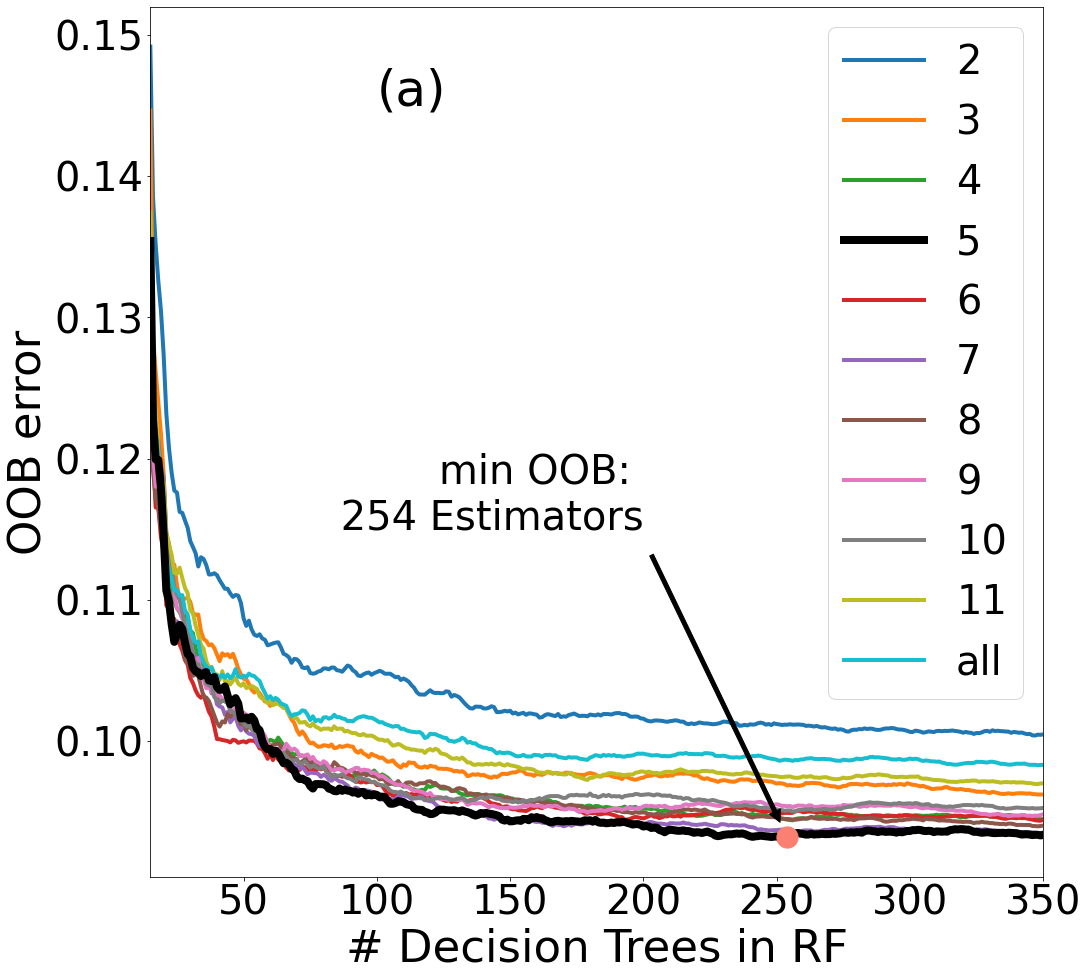
\includegraphics[width=0.95\linewidth, keepaspectratio=true]{./src/RF_oob_error}
		\caption{}
		\label{subfig:rfoob}
	\end{subfigure}
	\begin{subfigure}{0.5\linewidth}
		\centering
		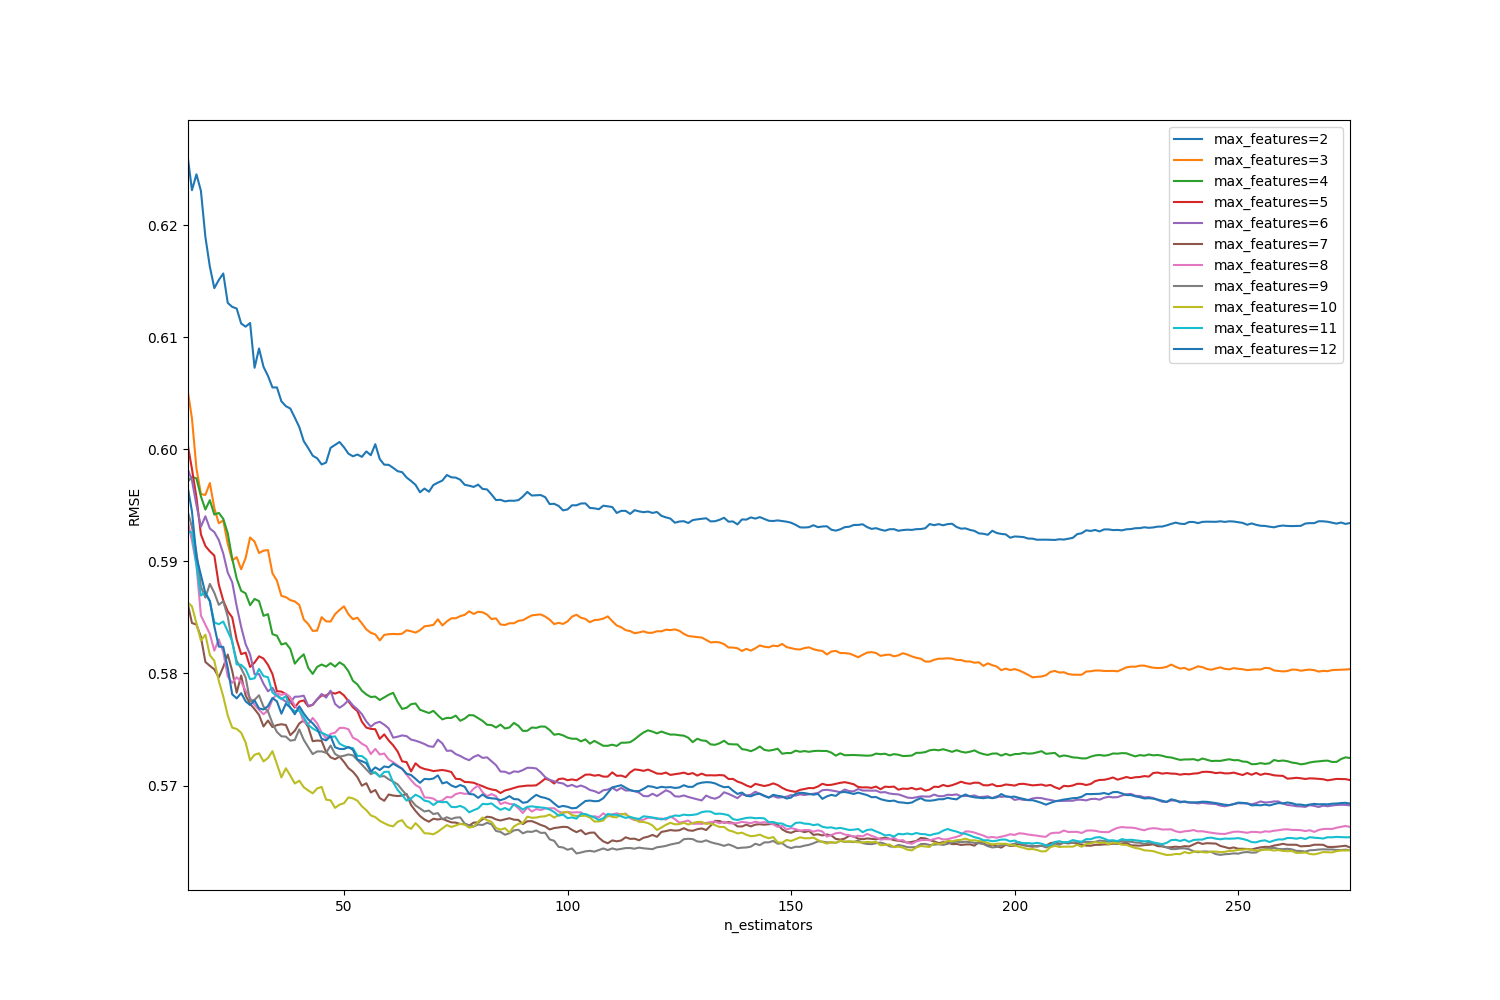
\includegraphics[width=0.95\linewidth, keepaspectratio=true]{./src/RF_RMSE_features_vs_num_estimators}
		\caption{}
		\label{subfig:rf_rmse}
	\end{subfigure}
	\caption{OOB error (a) and prediction quality (b) for Random Forests}
	\label{fig:RF_exp}
\end{figure}

The precise architecture of the RFs and ERTs was determined by grid searching across a domain of parameters (hidden leaf size, number of trees, split impurity size). The best preforming RF was that of \textcolor{green}{HYPEREPARAMS FOR RF} and that of the ERT was\textcolor{green}{HYPERPARAMETERS ERT}.
The results of the OOB error are visualized in Figure \ref{subfig:rfoob}, and the quality of performance in Figure~\ref{subfig:rf_rmse} as a function of the number of decision trees used to build the RF. Both plots compare the amount of features used to build the RF. From the OOB expereiment, we see that the RFs that made use of 6 to 11 features are all converge to relative same levels of OOB errors. These RFs indicate the folowing order of relevance of control parameters, where $x_i / x_j$ means that more often was $x_i$ ranked more important, but sometimes the RF chose $x_j$ ahead of $x_i$:
\begin{itemize}
	\item $I_p, \delta, \Gamma / q_{95}, a / B_T,  V_P / Z_{eff}, P_{NBI} /  P_{TOT}$ followed by very little relevance of $\Gamma_{SD}, P_{ICRH}, H, M_{eff}$
\end{itemize}

To see the power parameters ranked so low is quite surprising in comparison to their placement with GP and linear regressor methods of feature selection. 
Just like GPs, the 3 features that were consistently were ranked least important are $H, M_{eff},$ and $P_{ICRH}$.

When using permutation importance via permuting the cluster of features found in \ref{fig:corrshit}, it was found that removing the plasma volume $V_P$ and total power $P_{TOT}$ where the only parameters that could be removed that did end up improving the performance of RF's. The improvement was less than marginal, a decrease in the RMSE and MAE by $0.01$. However, this is an improvement overall, since the dimensionality of the feature space can be reduced for RF's, in addition to the methods of feature selection above, will result in quicker training cycles and faster prediction times overall. 

\begin{figure}
	\begin{subfigure}{0.5\linewidth}
		\centering
		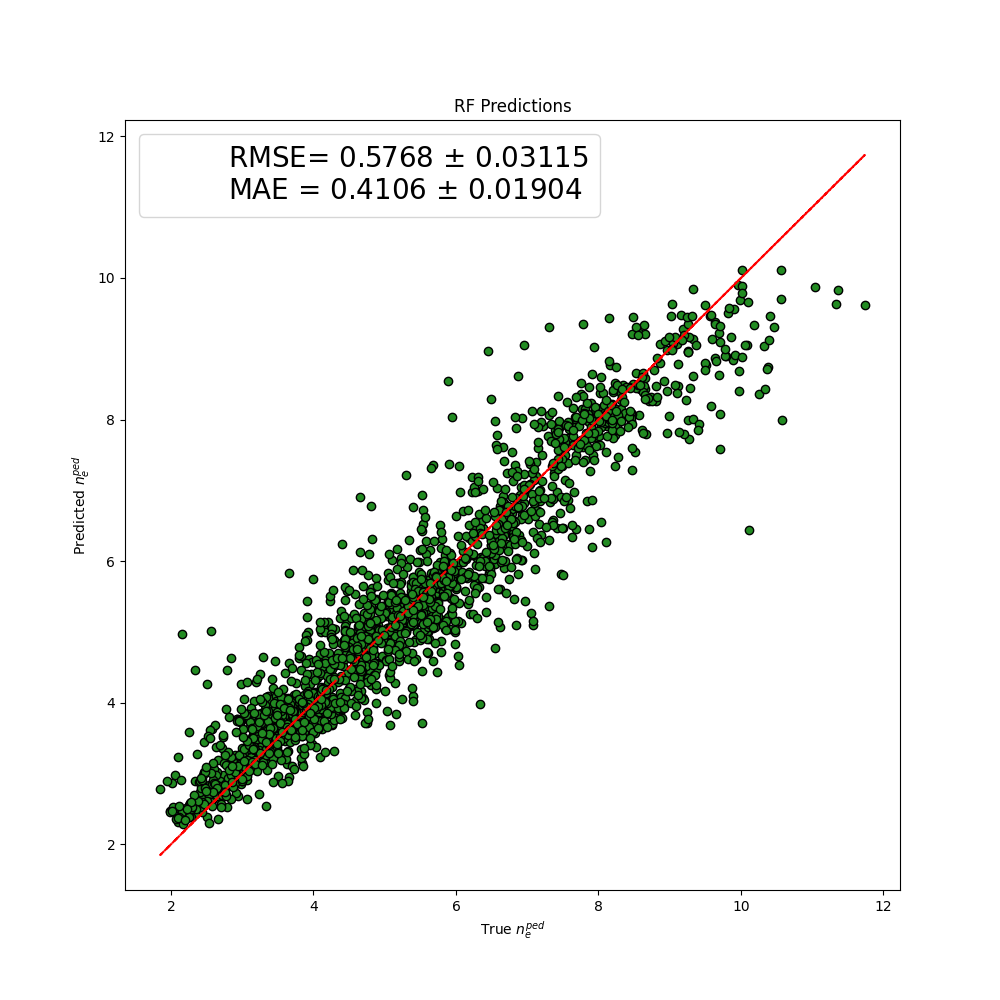
\includegraphics[width=0.99\linewidth, keepaspectratio=true]{./src/RF_predictions_and_uncert}
		\caption{}
		\label{subfig:RF_UQ}
	\end{subfigure}
	\begin{subfigure}{0.5\linewidth}
		\centering
		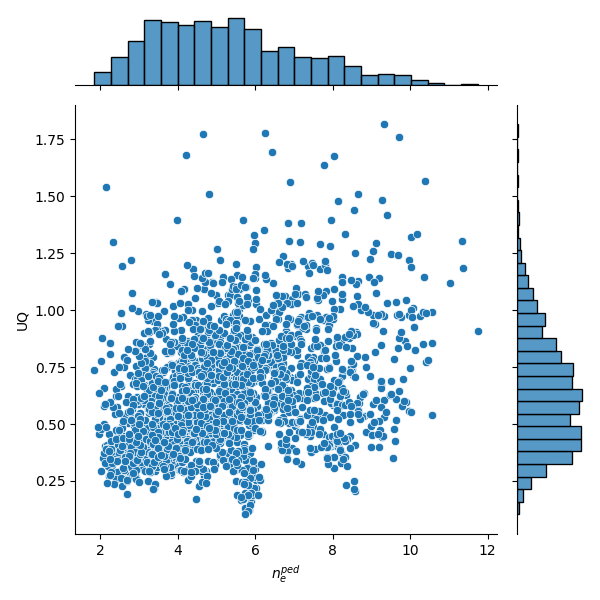
\includegraphics[width=0.99\linewidth, keepaspectratio=true]{./src/RF_UQ}
		\caption{}
		\label{subfig:RF_UQ2}
	\end{subfigure}
	\caption{}
	\label{fig:RF_Preds}
\end{figure}
In regards to the UQ of Random Forests, since there are $\approx 2000$ entries, attaching little error bars to each point estimate would not show much on a graph, therefore in Figure\ref{subfig:RF_UQ} I plot on the LHS the point predictions and on the RHS the determined uncertainty against the values of true $n_e^{ped}$. It is quite obvious that the uncertainty in prediction follows quite closely the distribution of entries for $n_e^{ped}$ as seen in \ref{subfig:RF_UQ2}, i.e., our uncertainty in an estimate is largely based on the amount of representation that estimate has in the dataset. 
\textcolor{red}{ERTs TBD}

\subsection{ANN's}
\textcolor{red}{TBD}

\subsection{Meta-Modeling}

\subsubsection{RFs and ERTs}
RF's split the leafs in each decision tree as to minimize the MSE, so by nature, the inclusion of synthesized values will not change the way the each tree is made unless it will improve predictions. It was seen that even with including up to 1000 synthesized entries (added during the CV split procedure, so essentially double the training entries were of $n_e^{ped} \geq 10.5$), no change in the performance of the RF was seen. 

\section{Discussion}\label{sec:discussion}
In predicting $n_e^{ped}$, it seems that parameters like $M_{eff}, H, P_{ICHR}$ have little to no relevance.

\end{comment}

\begin{comment}


\subsection{Uneccesary details / Appendix}

\section{Linear Regression}
Under the hood, linear regression uses inputs $\vec{x}$ to make an estimate $\hat{y}$ on what $y$, via the following prediction function:

\begin{equation} \label{eq:linreg}
	\hat{y} = f(\vec{x}) = \vec{w} \vec{x} + \epsilon
\end{equation}

where $\vec{w} = (w_1, w_2, \cdots, w_p)$ is a vector of parameters or coefficients that are multiplied by each feature $x_i$ before summing up the contributions from each feature, and $\epsilon$ is the irreducible error.
It is common to refer to the coefficients as \textit{weights} that determine how each control parameter affects the prediction of $n_e^{ped}$. If the coefficient is positive, then as that feature increases in value, then so will the prediction of $n_e^{ped}$, whereas if the coefficient is negative, then increasing the feature value will lead to a decrease in the prediction value. If the weight is 0, then the feature will play no role in the prediction, whereas if it is very large, it will dominate the effects on the prediction. The weight values are deterimned via ordinary least squares algorithm [SOURCE]. The general idea is to minimize the euclidian distance between the target and predictions using the mean squared error rewritten below.
\begin{equation}\label{eq:OLS}
	MSE_{OLS} = \frac{1}{N} \sum_i \left( y_i -  \sum_{j=1}^p x_{ij} w_j \right)^2
\end{equation}
Thus there exists an optimal set of weights for each of the features that minimize this cost function. It could be that the simple linear terms do not fully capture the relationship between $\vec{x}$ and $y$, and one would like to add polynomial terms to the prediction function \ref{eq:linreg}, and the polynomial terms would have their own coefficients. This is one way to increase a linear model's representational capacity, however at the same time increases the model complexity, and could potentially lead to overfitting. It is preferred to reduce model complexity and overfitting as much as possible without sacrificing performance. To reduce complexity without sacrificing performance, regularization is used. Regularization can be thought of as any modification one makes to a learning algorithm that is intended to reduce its generalization error, but not its training erro.  This can be done in the case of linear regression by adding a penalty term to the cost function; one such method, $L^1$ regualrization, or \textit{weight decay}, is preformed by comprimising both the MSE written above, and a the criterion $\mathbb{L}$ that expresses the preference for having smaller weights than the $L^1$ norm.
\begin{equation}
	\mathbb{L}(\vec{w})_{L1} = MSE_{OLS} +  \lambda |\vec{w}|;
\end{equation}
where $\lambda \in \mathbb{R}$ represents the regularization term and is chosen prior to the fitting procedure. For $\lambda =0$, the OLS cost function does not change.
Minimizing $\mathbb{L}(\vec{w})$ results in a choice of weights that balance well fitting of the data while keeping the weights as small as possible.
A regression model that minimizes this particular cost function is called a Lasso model. The neat trick with this form of regularization, is that it is possible for the weights of a certain features to reduce to near zero in order to achieve the lowest MSE. Weight coeficcients of control parameters that are contribute "less" to the regression function drop to zero, effectively acting as a form of \textit{feature selection}[SOURCE], deeming which control parameters are important for the linear regressor and its task of predicting $n_e^{ped}$.
In Section 3, I show which control imputs are deemed important by the Lasso procedure, as well as compare the scaling law to a linear regressor that uses the features determined by the Lasso as inputs.

\subsubsection{Baysian Linear Regression for UQ}
One of the downsides of linear regression, and most machine learning models, is that they produce point predictions of a quantity. In science, we are not only interested in a prediction, but also how uncertain we are in the prediction. For linear regressors, the point prediction can vary depending on the weights, thus any change to the weights will result in a change in the prediction. To quantify how certain we are with the choice of weights of a regressor is to quantify the uncertainty in its prediction. If each weight $w_i$ in $\vec{w}$ in \ref{eq:linreg} is a scalar quantity, this is quite difficult. However, if the weights were instead normal distributions, with the mean centered around the desired coefficient, then the uncertainty would be the spread of the weight's distribution. This is called Bayseian linear regression, which operates much like the above process.

\subsection{Gaussian Processes}
Instead of searching the space of possible coefficients that best parameterize the prediction function \ref{eq:linreg}, what if we lookd for the best prediction function to parameterize $n_e^{ped}$? This is the idea behind Gaussian Processes(GPs). For example, fitting a quadratic function using equation \ref{eq:linreg} would be futile, so by adding further polynomial terms one should converge to a more viable solution. But in the case of finding a prediction function for $n_e^{ped}$, we do not know what kind of function will give the best fit. The GP approach is thus a \textit{non-parametric} approach, and finds a distribution over the possible functions $f(x)$. Now there are a lot of functions that could fit $n_e^{ped}$, so by scaling $n_e^{ped}$ to have a mean of 0 and spread of 1, the domain of sample functions are reduced to those that produce outputs with similar mean and spread. Some of these functions may be very 'wiggly', i.e., they bounce from point to point quite quickly, whereas a smoother function ( not so 'wiggly'), is that which resembles splicing techniques. To specify the smoothness, a covariance matrix, or \textit{kernel} is used, such that values that are close together in input space will produce output values that are close together.  Lots of math goes into this, which can be found in the following [SOURCES]. Within the context of this thesis, I am interested in determining which kernel produces an optimal distribution of functions. In section 3, I show which kernels give the best performance score on predicting $n_e^{ped}$.

Just like with Lasso linear regression, the relevance of input variables of a fitted GP model can be determined, but intsead of the magnitude of the scaler weight coeficcient, it is instead the length-scale parameters of the kernel used (DEFINE LENGTH-SCALE BEFORE)[SOURCE]. In the context of bayesian modeling, this is called automatic relevance detmination [SOURCE]. Alternatively, feature selection for GP's can be done using sensitivty analysis, with detailed explaination of the math behind sensitivy analysis found in [SOURCE]. There are two types of sensitivity analysis used in this thesis, the first is through the use of  the Kullback-Leibler Divergence (KLD) [SOURCE]. The difference in KLD when an input $\vec{x}$ is altered with respect to a single feature $x_i$ will tell the predictive relevance; a large difference in the KLD indicates that the feature has high predictive relecance, and with low difference in KLD the feature has low predictive relevance. The second type of sensitivity analysis used in this thesis is teh Variance of the Posterior (VAR). VAR makes uses of the latent mean of a GP, and specifically looks at the variability of this latent mean when the value of a single feature is changed; large variability in the latent mean indicates that the feature is relevant in predicting $n_e^{ped}$, and low variability in the latent mean indicates it is not.

In section 3, I show which features are selected by GP's using ARD, KLD, and VAR for various kernels.

\subsubsection{UQ for GPs}
Fitting a GP yields a joint-gaussian group of functions, which when given an input of control parameters, each function within the group gives a prediction of $n_e^{ped}$, and the mean of all of these outputs is then the final point prediction of $n_e^{ped}$. The UQ is built into the GP in that the uncertainty in the mean point preidction is just the standard deviation of the outputs across all of the functions used in the mean. With GPs, not only is it possible to quantify the uncertainty in the prediction, but also to make use of the uncertainties in the data. To do this, \textcolor{blue}{need more detail about how this is possible}.

\subsection{Random Forests}
The intuition for random forests (RFs) is very different from that of the above mentioned regression techniques. For detailed information on what decision trees are and how they work well as when combined as RFs regressors, see [SOURCES]. A main difference in traditional regression tools and random forests is the way in which data is sampled to be fed to the regressor. RFs make use of the method of \textit{bootstrap aggregation}, in which the data is randomly sampled from the larger dataset to create the trees within the random forest. The method is a bit more complicated than just randomly sampling, but more can be read here [SOURCE]. In the context of this thesis, it is important to know that each tree in the RF uses a different sampled subset of data to manifest itself, i.e., not every tree is built using the same subset of data, and some entries will be contained in the fitting of the tree and some not.
Furthermore, in addition to randomly sampling the data points to create random subsets of data, RFs also sample random susbets of the features. The number of features to randomly select from the available control parameters set is chosen before fitting and is thus a hyperparameter. The features then chosen for each tree can be compared, and the relevance of the features is then quanitified from the number of trees that chose them vs how many trees in total there are in the forest \textcolor{blue}{describe how the relevance is chosen from the trees dropping out if they are shit}. In order to find the optimal number of features to use, I study the \textit{out-of-bag} (OOB) error. The OOB error is the average error for each prediction of a sample from the training set that is \textbf{not} contained in a tree[SOURCE]. The OOB error indicates how well a forest extrapolates the information, and a low OOB error refers to the RF that can best generalize predicting $n_e^{ped}$.
In Section 3, I compare the OOB error for different number of features used to determine the optimal number for RF, as well as discuss which features are selected in this process.

In addition to the out-of-bag error as an approach to feature selection, permutation importance (PI) can also be used. PI works particularly well for non-linear models like RFs and ERTs, and is defined as the decrease inamodel score when asingle feature value is randomly shuffled (corrupted). Similar to KLD, where a singular data entry is altered feature wise, PI instead shuffles the value of entire features and checks to see how the model reacts [SOURCE]. Permutating the feature space in this way yeilds the importance of a feature that is the models score when fitted on the shuffled dataset subtracted form the baseline score of the model fitten on the unperterbed case. However, when two features are strongly correlated, in the case of the power trio $P_{NBI}, P_{ICRH}, P_{TOT}$, the model will still have access to the feature via proxy with the correlated feature. To handle this, I employ a clustering technique in cluster correlated features based on their Spearman rank-order correelations, and then keep only one feature form each cluster. In Section 3 I show the results of the Spearman rank-order correlations by showing which parameters, when taken out from the list of input features, improve prediction quality.

\subsubsection{Extreme Random Trees}
All of the above semantics can be applied to Extreme Random Trees(ERTs). ERTs are slightly different from RF's, in that \textcolor{blue}{Describe ERTs and how they are different, advantages and disadvantages}

\subsubsection{UQ}
Within a RF there are $n$ decision trees built, and in order to quanitfify the uncertainty of the RF, I take the standard deviation of the prediction of each decision tree making up the RF. Additionally, one can use the ensemble method similar to that which is explained for ANN's later, in which the uncertainty in the ensemble becomes the uncertainty in the prediction, even further could one take the standard deviation of all the decision trees in the ensemble of random forests used.

\subsection{ANN's}
In this thesis, only feed forward networks are used for the prediction of $n_e^{ped}$.
The use feed-forward neural networks as a regresssion teqnique is no new task, and using a series of nested non-linear function to provide continous predictions on $n_e^{ped}$ makes this regression solution different only in method. T
\textcolor{blue}{TBD. }

\subsection{Meta-Modeling}
Another use of the uncertainties of each parameter is to generate synthesized values by using the measured parameter value as the mean of normal distribution and its uncertainty as the spread.
By sampling from the distribution of each parameter, it is possible to generate new 'synthesized' values. As seen in the next section, many models can predict well for $n_e^{ped} \leq 10$, but struggle for densities higher than that. Since ML the models above are very dependent on the data used to fit them, and consdiering that in the dataset there are less than 10 shots that have $n_e^{ped} \geq 10$, by including synthesized values in the fitting procedure the hope was that the models would be able to predict bettter on held out set that did not include the synthesized values.

\end{comment}
\bibliographystyle{unsrt}
\bibliography{biblioski}
\end{document}
